\documentclass[twoside, 12pt]{article}
\usepackage{Shapes}
\usepackage[utf8]{vietnam}
\usepackage{microtype}
\usepackage{mathtools,amssymb}
\usepackage{diagbox}
\usepackage{lmodern}
\usepackage{listings}
\usepackage{tikz}
\usepackage{tasks}
\usepackage{xcolor}
\usepackage{hyperref}
\usepackage{caption}
\usepackage{float}
%%%%%%%%%%%%
% \usepackage{indentfirst}
\setlength{\parindent}{0pt}
\usepackage{tikz}
\usepackage{pgfplots}
\usetikzlibrary{shapes.geometric, arrows}
\newcounter{example}[section]
\newenvironment{example}[1][]{\refstepcounter{example}\medskip
   \textbf{Ví dụ~\theexample : #1} \rmfamily}{\medskip}

\newcounter{defs}[subsection]
\newenvironment{defs}[1][]{\refstepcounter{defs}
   \textbf{Định nghĩa~\thesubsection.\thedefs : #1} \rmfamily}

\newcounter{clause}[subsection]
\newenvironment{clause}[1][]{\refstepcounter{clause}\medskip
   \textbf{Mệnh đề~\thesubsection.\theclause : #1} \rmfamily}{\medskip}
%%%%%%%%%%%%%%%%%%%

\usepackage{titlesec}
\usepackage{mdframed}

\usepackage{relsize}

\usepackage{mathptmx}
\usepackage{amsthm}
\usepackage{multicol}

\theoremstyle{definition}
\newtheorem{definition}{Định nghĩa}[section]

\theoremstyle{definition}
\newtheorem{theorem}{Định lý}[section]

\newtheorem*{remark}{Nhận xét}

\newtheorem{vd}{Ví dụ}[section]
\newtheorem{bt}{Bài tập}[section]
\newtheorem{tc}{Tính chất}[section]
\newtheorem{md}{Mệnh đề}[section]
\newtheorem{cy}{Chú ý}[section]
%%%%%%%%%%%%%%%%%%%


%\fancyhead[LO, RE]{Toán Tin 01 - k64}
%\fancyhead[LE, RO, font=\bfseries, color=HustRed]{MI4024 - Lớp 129852}
\definecolor{dkgreen}{rgb}{0,0.6,0}
\definecolor{Gray}{rgb}{0.5,0.5,0.5}
\definecolor{mauve}{rgb}{0.58,0,0.82}
\definecolor{cadmiumorange}{rgb}{0.93, 0.53, 0.18}
\definecolor{sami}{RGB}{1,90,143}
\lstdefinestyle{mystyle}{
	frame=shadowbox,
  language=SQL,
  aboveskip=3mm,
  belowskip=3mm,
  showstringspaces=false,
  columns=flexible,
  basicstyle={\normalsize\ttfamily},
  numbers=left,
  numberblanklines=true,
  numbersep=5pt,
  numberstyle=\tiny\color{gray},
  keywordstyle=\color{sami},
  morekeywords={USE},
  commentstyle=\color{dkgreen},
  stringstyle=\color{cadmiumorange},
  breaklines=true,
  breakatwhitespace=true,
  tabsize=2,
  keepspaces=true
}
\lstset{style=mystyle}
\title{Báo cáo cuối kỳ}

\subtitle{\begin{center}
    KHO DỮ LIỆU VÀ KINH DOANH THÔNG MINH\\
\end{center}\\Chủ đề:\\  Healthycare - Chăm sóc sức khỏe}
\author{
Nhóm thực hiện: & Nhóm 9 \\[0.3cm]
%Thành viên:\\
Nguyễn Thị Duyên & 20195866\\
Phạm Thị Hoa & 20195874\\
Trần Thị Hồng & 20195880\\
Phạm Thu Trang & 20195931\\
Trần Thị Hồng Vân & 20195941\\[0.3cm]
Lớp: &133598 - MI4214\\
Học kỳ: & 20212
}
\info{\textbf{Giảng viên hướng dẫn: ThS. Nguyễn Danh Tú} 
}
\logo[scale=0.62]{logotitle.png}



%---------------------------------------------------------------------
\newmdenv[linecolor=black,skipabove=\topsep,skipbelow=\topsep,      %|
leftmargin=-5pt,rightmargin=-5pt,                                   %|
innerleftmargin=5pt,innerrightmargin=5pt]{mybox}                    %|
%---------------------------------------------------------------------
\usepackage{indentfirst}
\begin{document}
\maketitlepage
\newpage
\tableofcontents
%%%%%%%%%%%%%%%%%
\newpage
\newpage
\newpage
\fontsize{22pt}{16pt}\selectfont
\begin{center}
    {\bfseries Lời mở đầu}
\end{center}
\fontsize{13pt}{16pt}\selectfont
\bigskip

Với sự phát triển khoa học kỹ thuật trên toàn cầu, nguồn dữ liệu thông tin khảo sát của mỗi một doanh nghiệp, tập đoàn ngày càng nhiều và tăng trưởng theo cấp số nhân. Với nhu cầu tiếp nhận, phân tích và xử lý dữ liệu dưới góc nhìn đa chiều và tổng hợp hiện nay, việc thống kê dòng dữ liệu là vô cùng cần thiết, từ đó khái niệm kho dữ liệu ra đời nhằm đảm lưu trữ đầy đủ dữ liệu cho bước phân tích tiếp theo và nâng cao tốc độ của các kết quả trả về của hệ thống. Cùng với Data Warehouse thì Dashboard cũng là một công cụ không thể thiếu trong các hoạt động kinh doanh, quản lý của tổ chức. Nhờ có Dashboard mà nhà quản trị có cái nhìn tổng quan, chi tiết và cụ thể cho hướng đi của doanh nghiệp.\\

Thế giới có nhịp độ nhanh ngày nay đã ảnh hưởng không nhỏ đến sức khỏe của chúng ta. Điều rất quan trọng là phải tiêu thụ thực phẩm lành mạnh và có một chế độ ăn uống cân bằng, tập luyện để giữ cho chúng ta khỏe mạnh về thể chất và tinh thần.\\

Dựa vào nhu cầu đó nhóm 9 quyết định chọn chủ đề HEALTH CARE để tìm
hiểu và báo cáo về các khảo sát sức khỏe của mọi người dựa vào các nhân tố ảnh hưởng đến sức khỏe như tuổi tác, các bệnh nền từ bộ dữ liệu của hệ thống giám sát yếu tố rủi ro hành vi BRFSS.\\

Chúng em xin gửi lời cảm ơn đến thầy ThS. Nguyễn Danh Tú đã hướng dẫn và đưa ra những góp ý cho nhóm hoàn thành đề tài.

\begin{minipage}{0.5\textwidth}
\end{minipage}
\hspace{0.5\textwidth}
\begin{minipage}{0.5\textwidth}
	\noindent\begin{center}
		\vspace{1cm}
		\textit{Hà Nội,ngày 26 tháng 7 năm 2022} \\
		Thay mặt nhóm báo cáo\\ \vspace{1cm}
		\textbf{Nhóm 9}\\
	\end{center}	
\end{minipage}

\bigskip

\newpage
%%%%%%%%%%%%%%
\newpage
\fontsize{22pt}{16pt}\selectfont
\begin{center}
    {\bfseries Đánh giá các thành viên}
\end{center}
\fontsize{13pt}{16pt}\selectfont
\bigskip

\subsection*{Các thành viên trong nhóm}
\begin{enumerate}
    \item  Nguyễn Thị Duyên - 20195866
    \item  Phạm Thị Hoa - 20195874
    \item  Trần Thị Hồng -20195880
    \item Phạm Thu Trang -20195931
    \item Trần Thị Hồng Vân - 20195941
\end{enumerate}

\subsection*{Đánh giá: }
\textbf{Bảng đánh giá các thành viên trong nhóm}
\begin{center}
            \begin{figure}[!h]
                \centering
                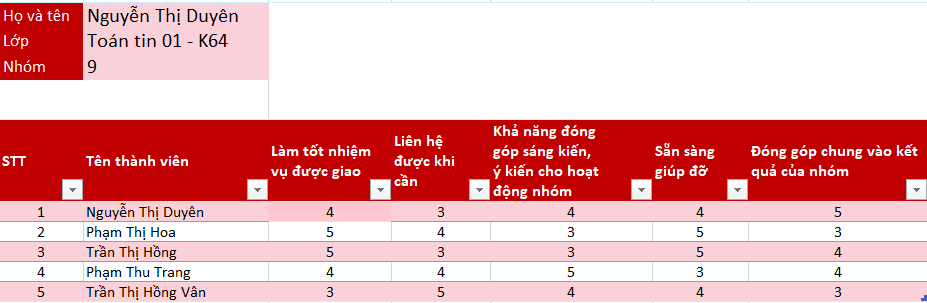
\includegraphics[scale = 0.8]{contents/Bảng đánh giá thành viên.PNG}
              \caption{Bảng đánh giá thành viên}
            \end{figure}
\end{center}
Trong quá trình hoạt động, các thành viên trong nhóm đều có tinh thần làm
việc tốt, hoàn thành tốt nhiệm vụ được giao và đều đóng góp vào trong kết quả
của nhóm, từ khâu chọn dữ liệu đến việc phân tích, xử lý dữ liệu và vẽ Dashboard.
Với tinh thần làm việc nhóm tốt, mọi người đã hoàn thành công việc đúng hạn và báo cáo Dưới đây là công sức của cả 5 thành viên đã cố gắng trong 16 tuần vừa qua.

\bigskip
\newpage
%%%%%%%%%%%%%%%%%%%%%%%%%%%%%%%%%%
\fontsize{22pt}{16pt}\selectfont
\begin{center}
    {\bfseries Tự đánh giá báo cáo nhóm}
\end{center}
\fontsize{13pt}{16pt}\selectfont
\bigskip
\begin{enumerate}
    \item \textbf{Mục tiêu và nội dung của báo cáo}
\begin{enumerate}
    \item \textbf{Mục tiêu:}\\
Sau khi hoàn thành báo cáo, chúng em sẽ nắm rõ được những khái niệm cơ bản về phân tích dữ liệu; hiểu được quy trình phân tích dữ liệu và triển khai vào công việc thực tiễn; Làm chủ được các công cụ trực quan hóa dữ liệu như Excel, Power BI và Hệ quản trị cơ sở dữ liệu để lựa chọn giải pháp tốt nhất trong thực tế.
\item \textbf{Nội dung của bài Báo cáo:}
\begin{itemize}[label=$-$]
    \item Tổng quan về Data Warehouse.
    \item Tổng quan về Heathycare
    \item Phân tích nghiệp vụ.
    \item Đưa ra requirement khi xây dựng kho dữ liệu.
    \item Kiến trúc Data Warehouse
    \item  Sơ đồ quá trình ETL và các nội dung ETL bằng Power Query và SQL
    \item Xử lý dữ liệu và vẽ sơ đồ dữ liệu OLTP
    \item  Sơ đồ các chiều dữ liệu
    \item Đưa dữ liệu từ cơ sở dữ liệu vào công cụ phân tích Power BI và OLAP hoá.
    \item Vẽ sơ đồ dữ liệu OLAP
    \item  Vẽ các dashboard theo chủ đề
    \item Phân tích các dashboard.
\end{itemize}
\end{enumerate}
\item \textbf{Kết quả đạt được:}
\begin{itemize}[label=$-$]
    \item  Hiểu được những kiến thức nền tảng cơ bản về Kho dữ liệu, Kinh doanh
thông minh, phân tích dữ liệu và phân tích kinh doanh. Bên cạnh đó xây dựng được kiến trúc của kho dữ liệu.
    \item  Nắm rõ được quy trình phân tích dữ liệu.
    \item Phân tích và thiết kế được các mô hình của hệ thống mới.
    \item Làm chủ được một số công cụ trực quan hóa dữ liệu như Excel, Power BI.
    \item Khảo sát và làm việc trên bộ dữ liệu thực tế
    \item Xây dựng được kiến trúc kho dữ liệu ứng với bài toán thực tế của nhóm.
    \item ETL dữ liệu trên các công cụ Excel, Power Query
    \item Vẽ được sơ đồ OLTP
    \item Xác định được các chiều phân tích của bài toán
    \item  Xây dựng được mô hình dữ liệu OLAP và đưa vào công cụ trực quan hóa Power BI.
    \item Xây dựng được các dashboard phân tích và tổng quan.
    \item Phân tích được các dashboard theo các chiều dữ liệu đã xác định.
    \item Tiếp cận đến các công cụ mới để phân tích dữ liệu và xây dựng DW
như SQL Server Analysis Service...
\end{itemize}
\item \textbf{Nội dung chưa làm được:}
\begin{itemize}[label=$-$]
    \item Chưa xử lý thành thạo bộ dữ liệu kích thước lớn, và còn thiếu dữ liệu ban đầu.
    \item Sử dụng công cụ trực quan hóa Power BI chưa được chuyên nghiệp, các Dashboard chưa phân tích sâu các chiều dữ liệu.
\end{itemize}
\item \textbf{Bài học thu được:}
\begin{itemize}[label=$-$]
    \item Việc xây dựng kho dữ liệu là vô cùng cần thiết cho mục đích phân tích dữ liệu.
    \item Dữ liệu trong thực tế không phải lúc nào cũng được chuẩn hóa theo một
quy tắc và không dữ liệu nào là hoàn hảo. Vì vậy luôn cần phải xử lý
trước khi đưa vào hệ thống.
\item Quá trình ETL dữ liệu rất quan trọng và tốn nhiều thời gian nên đòi
hỏi cần phải tập trung quan tâm thực hiện. Cần nghiên cứu bộ dữ liệu
một cách tỉ mỉ để xử lý dữ liệu một cách đúng đắn để tránh xảy ra sai
sót và mất dữ liệu
\item Dữ liệu có kích thước lớn gây ảnh hưởng đến thời gian chạy của máy
tính, cần chọn máy có cấu hình phù hợp cho việc xử lý và phân tích.
Và có thể chia nhỏ các file để dễ dàng thực hiện.
\item  Kiến thức nghiệp vụ của mỗi quy trình là vô cùng quan trọng, vì khi
hiểu được nghiệp vụ chúng ta mới có thể xây dựng được một hệ thống
BI đúng và hiệu quả. Vì vậy, đầu tiên cần phải khảo sát thật kỹ nghiệp
vụ của từng quy trình hoạt động.
\item  Mô hình dữ liệu đa chiều giúp phân tích dữ liệu trên nhiều góc nhìn
khác nhau, và có thể phân cấp.
\item Các dashboard nên được xây dựng theo hướng chủ đề, phải đảm bảo
tính logic và thẩm mỹ.
\end{itemize}
   
%\end{enumerate}
\end{enumerate}
\newpage
%%%%%%%%%%%%%%%%%%%%%%%%%%%%%%%%%%
%\tableofcontents
\newpage
\listoffigures
%\newpage
%\listoftables


\newpage
\section{Tổng quan về Data Warehouse}
\subsection{Khái niệm:}
Kho dữ liệu (Data Warehouse) được hiểu là một tập hợp các dữ liệu tương đối ổn định (không hay thay đổi), cập nhật theo thời gian, được tích hợp theo hướng chủ đề nhằm hỗ trợ quá trình tạo quyết định về mặt quản lý (W.H. Inmon).\\

Kho dữ liệu về bản chất là một cơ sở dữ liệu bình thường, các hệ quản trị cơ sở dữ liệu quản lý và lưu trữ nó như các cơ sở dữ liệu thông thường. Tuy nhiên, nó có thể quản lý dữ liệu lớn và hỗ trợ truy vấn. Nên điểm khác biệt giữa kho dữ liệu và cơ sở dữ liệu là ở quan niệm, cách nhìn nhận vấn đề.

\subsection{Đặc tính:}
\begin{enumerate}
    \item Hướng chủ đề: Cung cấp một khung nhìn đơn giản và súc tích xung quanh các sự kiện của các chủ đề ứng với mỗi loại tổ chức. Kho dữ liệu được thiết kế để hỗ trợ việc phân tích dữ liệu và hỗ trợ ra quyết định sau khi loại bỏ những dữ liệu không hữu ích.
    \item Tính tích hợp: Là đặc tính quan trọng nhất. Khi dữ liệu từ nhiều nguồn khác nhau đưa vào kho dữ liệu, chúng sẽ được chuyển đổi, định dạng lạ,.. để đảm bảo sự đồng nhất trong các quy ước tên, cấu trúc mã hóa, các đơn vị đo, thuộc tính,... giữa các nguồn khác nhau.
    \item Gắn thời gian và có tính lịch sử: Dữ liệu trong kho dữ liệu bao gồm cả quá khứ và hiện tại. Mỗi dữ liệu trong kho dữ liệu đều được gắn với thời gian và có tính lịch sử.
    \item Chỉ đọc, không biến động: Là một lưu trữ vật lý của dữ liệu được chuyển đổi từ môi trường tác nghiệp. Kho dữ liệu tách rời với môi trường tác nghiệp, nên dữ liệu trong đó là dữ liệu chỉ đọc, không chỉnh sửa hoặc thêm mới.
\end{enumerate}
\subsection{Lợi ích}
\begin{itemize}[label=$-$]
    \item Dữ liệu sau khi đưa vào kho dữ liệu đều tuần theo những quy tắc thống nhất.
    \item Dữ liệu được tổ chức tạo thuận lợi cho việc truy vấn phân tích và tạo tiền đề để đưa ra những quyết định có ảnh hưởng lớn.
    \item Cải thiện tính bảo mật và hiệu suất mà không cần tách động tới hệ thống dữ liệu gốc.
    \item Công việc kinh doanh trở nên thông minh hơn, nâng cao dịch vụ khách hàng.
\end{itemize}

\subsection{Kiến trúc:}
\subsubsection{Phân loại kiến trúc:}
Phụ thuộc rất nhiều vào vị trí của từng bộ phận trong tổ chức. Các kiến trúc phổ biến của kho dữ liệu bao gồm:
\begin{enumerate}
    \item \textbf{Kiến trúc cơ bản:}
    Kiến trúc cơ bản rất ít được sử dụng trong thực tế. Mặc dù, kiến trúc này loại bỏ dư thừa dữ liệu giúp giảm thiểu lượng dữ liệu được lưu trữ nhưng không phù hợp với các doanh nghiệp có yêu cầu dữ liệu phức tạp và nhiều nguồn dữ liệu. Trong kiến trúc cơ bản chỉ có tầng nguồn là tầng có sẵn về mặt vật lý. Kho dữ liệu của kiến trúc này là ảo tức nó được xây dựng dưới dạng một cái nhìn đa chiều về dữ liệu hoạt động và được tạo bởi phần mềm trung gian cụ thể hoặc một lớp xử lý trung gian.
    \begin{center}
            \begin{figure}[!h]
                \centering
                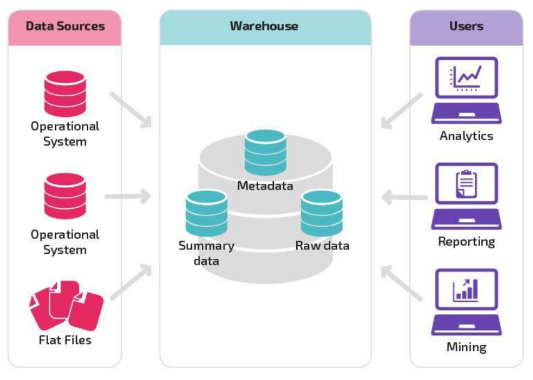
\includegraphics[scale = 1]{figures/Duyen/Kiến trúc kho dl cơ bản.PNG}
              \caption{Kiến trúc kho dl cơ bản}
            \end{figure}
\end{center}
    \item \textbf{Kiến trúc với vùng tập kết dữ liệu (Staging Area):} Kiến trúc này cung cấp thông tin luôn ở chất lượng tốt, ngay cả khi quyền truy cập vào các nguồn bị từ chối tạm thời vì lý do kỹ thuật hoặc tổ chức; truy vấn phân tích kho dữ liệu không ảnh hưởng đến việc quản lý các giao dịch, độ tin cậy cao, kho dữ liệu được cấu trúc logic theo mô hình đa chiều, kho dữ liệu có thể sử dụng các giải pháp thiết kế cụ thể để tối ưu hóa hiệu suất của các ứng dụng phân tích và báo cáo.
    \newpage
    \begin{center}
            \begin{figure}[!h]
                \centering
                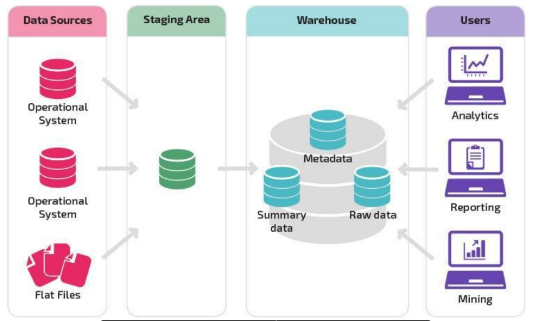
\includegraphics[scale = 1]{figures/Duyen/Kiến trúc kho dữ liệu vs Staging Area.PNG}
              \caption{Kiến trúc kho dữ liệu vs Staging Area}
            \end{figure}
\end{center}
    \item \textbf{Kiến trúc với vùng tập kết dữ liệu (Staging Area) và kho dữ liệu chủ đề (Data Marts):}
    Đây là kiến trúc phổ biến nhất trong ba loại. Ưu điểm chính của tầng tập kết dữ liệu (Staging Area) là tạo ra một mô hình dữ liệu tham chiếu chung cho cả doanh nghiệp. Đồng thời, tách biệt rõ ràng các vấn đề khai thác và tích hợp dữ liệu nguồn với các vấn đề của tổng thể kho dữ liệu. Đáng chú ý, tầng tập kết dữ liệu cũng được sử dụng trực tiếp để hoàn thành tốt một số nhiệm vụ hoạt động. Bên cạnh đó, kho dữ liệu chủ đề (Data Mart) giúp dữ liệu được truy cập dễ dàng hơn và cải thiện hiệu suất hệ thống.
     \begin{center}
            \begin{figure}[!h]
                \centering
                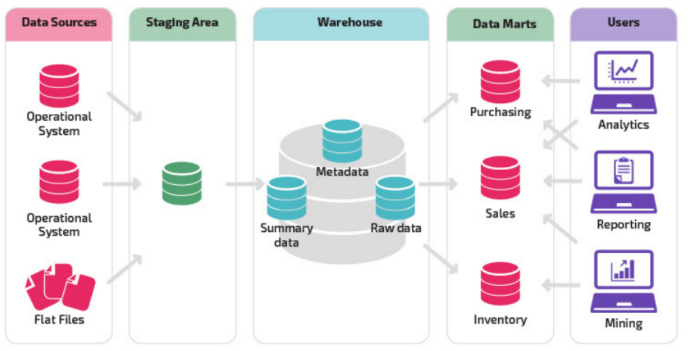
\includegraphics[scale = 1]{figures/Duyen/Kiến trúc kho dl với Staging và Data Marts.PNG}
              \caption{Kiến trúc kho dl với Staging và Data Marts}
            \end{figure}
    \end{center}
\end{enumerate}
    \subsubsection{Nguồn dữ liệu}
    Nguồn dữ liệu của kho dữ liệu rất đa dạng:
    \begin{itemize}[label=$-$]
        \item Dữ liệu từ các hệ thống tác nghiệp.
        \item Hệ thống kế thừa.
        \item Các nguồn dữ liệu bên ngoài.
    \end{itemize}
\subsubsection{Tập kết dữ liệu}
Tập kết dữ liệu (Data Staging) là nơi lưu trữ trung gian được sử dụng để xử lý dữ liệu trong thời gian chiết xuất, chuyển đổi và tải (ETL) quá trình. Dữ liệu tại đây có thể bị xóa trước khi chạy quy trình ETL hoặc ngay sau khi hoàn thành thành công quy trình ETL.\\
    Tuy nhiên, trong một số trường hợp Data Staging được thiết kế để
lưu giữ dữ liệu trong thời gian dài cho các mục đích lưu trữ hoặc xử lý sự cố.
\subsubsection{Công cụ trích xuất, chuyển đổi và tải dữ liệu}
Quy trình ETL được thiết kế phù hợp trích xuất dữ liệu từ hệ thống nguồn, thực thi các tiêu chuẩn về chất lượng và tính nhất quán của dữ liệu, tuân thủ dữ liệu để các nguồn riêng biệt có thể được sử dụng cùng nhau và cuối cùng cung cấp dữ liệu ở định dạng sẵn sàng trình bày để
các nhà phát triển ứng dụng có thể xây dựng ứng dụng và người dùng cuối có thể đưa ra quyết định.
\begin{enumerate}
    \item \textbf{Trích xuất (Extract):}
    Trích xuất dữ liệu một cách tạo tiền đề cho sự thành công của các
    quy trình tiếp theo. Hầu hết các dự án kho dữ liệu kết hợp dữ liệu từ các hệ thống nguồn khác nhau. Mỗi hệ thống riêng biệt cũng có thể sử dụng một tổ chức và/hoặc định dạng dữ liệu khác nhau. Việc truyền trực tuyến nguồn dữ liệu được trích xuất và tải nhanh chóng
    đến cơ sở dữ liệu đích là một cách khác để thực hiện ETL khi không cần lưu trữ dữ liệu trung gian. Quá trình trích xuất nhằm xác thực dữ liệu xem được lấy từ các nguồn có các giá trị chính xác hay không.
    \item \textbf{Biến đổi (Transform):}
    Trong giai đoạn chuyển đổi dữ liệu , một loạt các quy tắc hoặc chức năng được áp dụng cho dữ liệu được trích xuất để chuẩn bị cho việc tải vào mục tiêu cuối cùng. Một chức năng quan trọng của chuyển đổi là làm sạch dữ liệu, nhằm chuyển dữ liệu "thích hợp"đến mục tiêu. Việc tương tác giữa các hệ thống khác nhau gặp cản trở do các bộ ký tự có thể có sẵn trong hệ thống này nhưng có thể không có ở các hệ thống khác.
    \item \textbf{Load:}
    Tùy thuộc vào yêu cầu của tổ chức, quá trình tải dữ liệu rất khác nhau. Một số kho dữ liệu có thể ghi đè thông tin hiện có bằng thông tin tích lũy; cập nhật dữ liệu trích xuất thường xuyên được thực hiện theo chu kỳ. Các kho dữ liệu khác (hoặc thậm chí các phần khác của cùng một kho dữ liệu) có thể thêm dữ liệu mới ở dạng lịch sử theo các khoảng thời gian đều đặn. Thời gian và phạm vi thay thế hoặc kết nối thêm là các lựa chọn thiết kế chiến lược phụ thuộc vào thời gian có sẵn và nhu cầu của doanh nghiệp. Các hệ thống phức tạp hơn có thể duy trì lịch sử và dấu vết kiểm tra tất cả các thay đổi đối với dữ liệu được tải vào kho dữ liệu.\\
    Khi giai đoạn tải tương tác với cơ sở dữ liệu, các ràng buộc được xác định trong lược đồ cơ sở dữ liệu - cũng như trong các trình kích hoạt được kích hoạt khi tải dữ liệu - áp dụng. Ví dụ: Tính duy nhất, tính toàn vẹn tham chiếu, các trường bắt buộc), cũng góp phần vào hiệu suất chất lượng dữ liệu tổng thể của quy trình ETL.
\end{enumerate}
\subsubsection{Siêu dữ liệu}
Siêu dữ liệu (Metadata) lưu các định nghĩa logic các bảng, thuộc tính của kho dữ liệu, tên các nguồn dữ liệu tác nghiệp, định nghĩa vật lý các bảng và các cột.
\subsubsection{Kho dữ liệu chủ đề}
Kho dữ liệu chủ đề (Data Mart) có những đặc điểm giống với kho dữ liệu (Data Warehouse) nhưng với quy mô nhỏ hơn và lưu trữ dữ liệu về một lĩnh vực, một chuyên ngành. Các kho dữ liệu chủ đề có thể được hình thành từ một tập con dữ liệu của kho dữ liệu hoặc cũng có thể được
xây dựng độc lập và sau khi xây dựng xong, các kho dữ liệu chủ đề có thể được kết nối tích hợp lại với nhau tạo thành kho dữ liệu. Vì vậy có thể xây dựng kho dữ liệu bắt đầu bằng việc xây dựng các kho dữ liệu chủ đề hay ngược lại xây dựng kho dữ liệu trước sau đó tạo ra các kho dữ
liệu chủ đề.
\subsubsection{Các công cụ và nền tảng hỗ trợ}
\begin{itemize}[label=$-$]
    \item Hệ quản trị CSDL: MySQL, Oracle, Microsoft SQL Server, MariaDB,..
    \item Trực quan hoá dữ liệu, tạo báo cáo (Report, Dashboard): Power BI, Tableau,...
    \item Phân tích dữ liệu: Python, R, SAS, Excel. Orange...
\end{itemize}
\subsection{Kiến trúc khối và Các dạng lược đồ dữ liệu đa chiều}
\subsubsection{Mô hình dữ liệu đa chiều}
Data Warehouse và các hệ thông OLAP được xây dựng theo mô hình dữ liệu đa chiều. Dữ liệu trong kho dữ liệu được thể hiện dưới dạng đa chiều gọi là khối (Cube). Mỗi chiều mô tả một đặc trưng nào đó của dữ liệu. (Nếu số chiều dữ liệu lớn hơn 3, gọi là Hyper Cube).
\begin{enumerate}
    \item \textbf{Chiều (Dimension) \& Độ đo (Measure)}
    \begin{itemize}[label=$-$]
        \item Chiều cung cấp các thông tin, ngữ cảnh của bảng Fact.
        \item Độ đo là đại lượng có thể tính toán được trên các thuộc tính của bảng Fact.
    \end{itemize}
    \item \textbf{Cây phân cấp \& Số liệu tổng hợp}
    \begin{itemize}[label=$-$]
        \item Mức độ chi tiết của các tiêu chí thể hiện cho người dùng được gọi là mức dữ liệu, được quyết định bằng việc kết hợp các mức dữ liệu của từng phân lớp.
        \item Số liệu tổng hợp: Việc tổng hợp số liệu xảy ra khi người dùng thay đổi mức chi tiết của dữ liệu lấy ra từ Cube, bằng cách duyệt qua cây phân cấp.
    \end{itemize}
    \item  \textbf{Các mô hình thiết kế Date Warehouse}
    \begin{itemize}[label=$-$]
        \item OLAP kiểu quan hệ (Relational OLAP $\sim$ ROLAP)
        \item OLAP kiểu đa chiều (Multi-dimensional OLAP $\sim$ MOLAP)
        \item OLAP kết hợp (Hybird OLAP HOLAP = ROLAP + MOLAP)
    \end{itemize}
    \begin{center}
            \begin{figure}[!h]
                \centering
                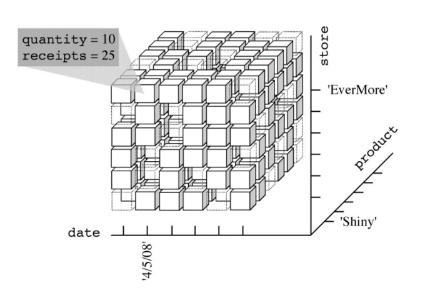
\includegraphics[scale = 1]{figures/Duyen/Minh họa khối dữ liệu.PNG}
              \caption{Minh họa khối dữ liệu}
            \end{figure}
\end{center}
\end{enumerate}
\subsubsection{Lược đồ dữ liệu đa chiều}
\begin{enumerate}
\item \textbf{Lược đồ hình sao}\\
Gồm 1 bảng Fact nằm ở trung tâm và những bảng Dimension bao quanh. Các câu hỏi nhằm vào bảng Fact và được cấu trúc bởi các bảng Dimension.
\begin{itemize}
    \item  Ưu điểm: Bảng Fact, Dimension được mô tả rõ ràng, dễ hiểu. Bảng Dim chứa dữ liệu tĩnh, và bảng Fact chứa dữ liệu động được nạp bằng các thao tác. Khoá của Fact được tạo bởi khoá của các bảng Dim. Nghĩa là khoá chính của các bảng Dim chính là khoá ngoại của bảng Fact.
    \item Nhược điểm: Dữ liệu không được chuẩn hoá
\end{itemize}
\item \textbf{Lược đồ hình bông tuyết}\\
Lược đồ hình bông tuyết là một sự mở rộng của lược đồ hình sao tại đó mỗi "cánh ngôi sao". Các chiều được cấu trúc rõ ràng. Bảng Dimension được chia thành hai chiều: chính và phụ.
\begin{itemize}
    \item Ưu điểm: Số chiều được phân cấp thể hiện dạng chuẩn của bảng Dimension.
    \item Nhược điểm: Cấu trúc phi dạng chuẩn của lược đồ hình sao phù hợp hơn cho việc duyệt các chiều.
\end{itemize}
\item \textbf{Lược đồ ngân hà}\\
Lược đồ ngân hà được hình thành nhờ sự kết hợp giữa lược đồ hình sao và lược đồ hình bông tuyết. Lược đồ này chứa nhiều bảng Fact sử dụng chung một số bảng Dim và là sự kết hợp của nhiều Data Mart.
\end{enumerate}
\newpage
\section{Tổng quan về BI}
\subsection{Khái niệm}
Kinh doanh thông minh (Business Intelligence - BI) là quy trình/hệ thống công nghệ cho phép phân tích và thể hiện thông tin giúp cho các nhà quản lý và người sử dụng của tổ chức đưa ra các quyết định phù hợp.\\
Kinh doanh thông minh bao gồm một loạt các công cụ, ứng dụng và phương thức cho phép các tổ chức thu thập thông tin từ các hệ thống nội bộ và bên ngoài; chuẩn bị sẵn sàng cho việc phân tích, phát triển và chạy các truy vấn đối với dữ liệu, tạo các báo cáo, bảng điều khiển và hình ảnh hóa dữ liệu để cung cấp kết quả phân tích cho những người sử dụng và những người ra quyết đinh.
\subsection{Các bước trong quy trình kinh doanh thông minh}
\begin{center}
            \begin{figure}[!h]
                \centering
                
\includegraphics[scale = 1]{figures/Duyen/Quy trình kinh doanh thông minh.PNG}
              \caption{Quy trình kinh doanh thông minh}
            \end{figure}
\end{center}
\newpage
\begin{itemize}[label=$-$]
    \item \textbf{ Nguồn dữ liệu (Data Source)} là vị trí bắt nguồn dữ liệu đang được sử dụng. 
    Nguồn dữ liệu có thể là vị trí ban đầu nơi dữ liệu được sinh ra hoặc nơi thông tin vật lý được số hóa lần đầu tiên, tuy nhiên, ngay cả những dữ liệu tinh tế nhất cũng có thể đóng vai trò là nguồn, miễn là một quy trình khác truy cập và sử dụng nó. Cụ thể, nguồn dữ liệu có thể là một cơ sở dữ liệu đến từ các hệ quản trị cơ sở dữ liệu MySQL, SQL, Oracle, MSSQL, một tệp phẳng, các phép đo trực tiếp từ các thiết bị vật lý, dữ liệu web cóp nhặt hoặc bất kỳ dịch vụ dữ liệu trực tuyến và tĩnh nào có rất nhiều trên internet...
    \item \textbf{Kho dữ liệu (Data Warehouse)} là cơ sở dữ liệu được thiết kế theo mô hình Online Analytical Processing (OLAP), dữ liệu trong data warehouse chỉ có thể đọc, không được ghi hay xóa mà chỉ được update bởi gói ETL chuyển đổi dữ liệu từ Data Sources vào Data Warehouse.
    \item \textbf{Khám phá dữ liệu (Data Exploration)} là bước đầu tiên trong phân tích dữ liệu, trong đó người dùng khám phá một tập dữ liệu lớn theo cách không có cấu trúc để khám phá các mẫu, đặc điểm và điểm quan tâm ban đầu.Khám phá dữ liệu tạo ra các truy vấn, báo cáo, biểu đồ phân tích, thống kê từ mô hình dữ liệu OLAP ở Kho dữ liệu.
    \item \textbf{Khác dữ liệu (Data mining)} là quá trình phân tích khối lượng lớn dữ liệu để khám phá thông tin kinh doanh giúp các công ty giải quyết vấn đề, giảm thiểu rủi ro và nắm bắt cơ hội mới.
\end{itemize}
\subsection{Lợi ích}
Những lợi ích chính mà doanh nghiệp có thể nhận được từ các ứng dụng BI:
\begin{itemize}[label=$-$]
    \item Tăng tốc và cải thiện việc ra quyết định
    \item Tối ưu hóa quy trình kinh doanh nội bộ
    \item Phát hiện các vấn đề kinh doanh cần được giải quyết
    \item Xác định các xu hướng kinh doanh và thị trường mới nổi
    \item Phát triển các chiến lược kinh doanh mạnh mẽ hơn
    \item Thúc đẩy doanh số bán hàng cao hơn và doanh thu mới
    \item Đạt được lợi thế cạnh tranh so với các công ty đối thủ
\end{itemize}
\newpage
Một số công cụ thông dụng hiện nay:
\begin{enumerate}
    \item Power BI
    \item Oracle BI
    \item QlikView
    \item Spago
    \item Pentaho
    \item IBM Cognos
\end{enumerate}
\subsection{ Công cụ trực quan hóa dữ liệu Power BI}
\subsubsection{Giới thiệu chung}
Power BI được ra đời vào năm 2011, được phát triển bởi Microsoft, sau đó nó được đưa vào sử dụng chính thức vào năm 2015. Power BI tập hợp rất nhiều các dịch vụ về phần mềm, các ứng dụng, các trình kết nối hoạt động song song cùng nhau để biến đổi các nguồn dữ liệu từ nhiều nguồn khác nhau thành các thông tin chi tiết liền mạch và trực quan. Power Bi được phát triển, sử dụng trên nền tảng Desktop, Website Service và Mobile App, nó hoàn toàn thân thiện và dễ dàng thích ứng với mọi người dùng mặc dù mỗi người đều có những nhu cầu khác nhau.
\subsubsection{ Các chức năng của Power BI}

\textbf{Kết nối dữ liệu từ nhiều nguồn}\\
Chúng ta có thể truy cập dữ liệu từ nhiều nguồn khác nhau dựa trên nền
tảng Power BI, bao gồm các nguồn như sau:
\begin{itemize}[label=$-$]
    \item File: các dạng Excel, Text/CSV, XML, JSON, Folder, PDF, SharePoint folder.
    \item Database: SQL Server database, Access database, Oracle database, IBM Db2 database, MySQL. . .
    \item Power Platform: Power BI datasets, Power BI dataflows, Common Data Service. . .
    \item Azure
    \item Online Services: SharePoint Online List, Microsoft Exchange Online, Dy-namics 365...
\begin{center}
            \begin{figure}[!h]
                \centering
                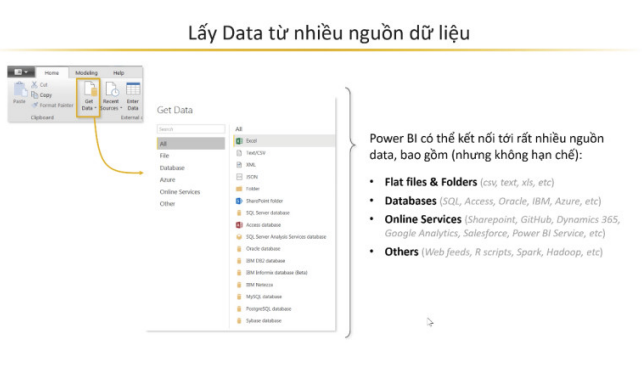
\includegraphics[scale = 1]{figures/Duyen/Kết nối dữ liệu trong PBI.PNG}
              \caption{Kết nối dữ liệu trong PBI}
            \end{figure}
\end{center}
\end{itemize}
\newpage
\textbf{Tiền xử lý dữ liệu}\\
Hầu hết trong doanh nghiệp, dữ liệu thu thập được đều đã trải qua quá trình tiền xử lý dữ liệu để có thể sẵn sàng sử dụng tạo ra các báo cáo. Trong quá trình tiền xử lý dữ liệu, các dữ liệu được trích xuất từ một nguồn dữ liệu, sau đó được chuyển đổi, xác thực, chuẩn hóa, sửa chữa, kiểm tra và cuối cùng được tải vào kho dữ liệu.
\begin{center}
            \begin{figure}[!h]
                \centering
                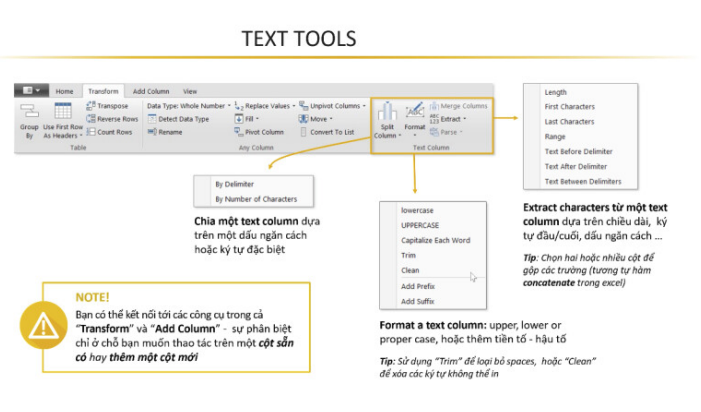
\includegraphics[scale = 1]{figures/Duyen/Tiền xử lý dữ liệu trong PBI.PNG}
              \caption{Kết nối dữ liệu trong PBI}
            \end{figure}
\end{center}
\newpage
Quy trình tiền xử lý dữ liệu được thực hiện bởi các ứng dụng như SQL Server Integration Services (SSIS) hoặc các công cụ của bên thứ ba khác. Tuy nhiên, trong một số doanh nghiệp, công việc tiền xử lý dữ liệu được thực hiện ngay trong Excel, được gọi là chuyển đổi dữ liệu. Tuy nhiên, quy trình ETL trong Excel là một quy trình thủ công, mất nhiều thời gian và khó có thể tự động hóa. \\
Vì thế Microsoft đã tạo ra công cụ để có thể làm cho quá trình này trở nên nhanh và dễ dàng hơn nhiều đó là Power Query, Power BI Desktop. Hai công cụ này cung cấp cho người dùng khả năng tự động hóa quá trình nhập, chuyển đổi và tải dữ liệu vào các bảng nội bộ trong Power BI, sau đó có thể được sử dụng làm nguồn cho các báo cáo hay dashboard của Power BI. Vì Power Query duy trì bản ghi từng bước của mọi hành động được thực hiện để nhập, chuyển đổi và tải dữ liệu, các bước này sẽ được lặp lại khi có thêm dữ liệu được thêm vào.
\textbf{Mô hình hóa dữ liệu (Data modeling)}
Mô hình hóa dữ liệu là quá trình tạo ra một biểu diễn trực quan của toàn bộ hệ thống thông tin hoặc các bộ phận của nó để giao tiếp các kết nối giữa các điểm và cấu trúc dữ liệu. Mục đích là minh họa các loại dữ liệu được sử dụng và lưu trữ trong hệ thống, mối quan hệ giữa các loại dữ liệu này, cách dữ liệu có thể được nhóm và tổ chức cũng như các định dạng và thuộc tính của nó.\\
Dữ liệu có thể được mô hình hóa ở nhiều mức độ trừu tượng khác nhau.
Quá trình bắt đầu bằng cách thu thập thông tin về các yêu cầu kinh doanh từ các bên liên quan và người dùng cuối. Các quy tắc nghiệp vụ này sau đó được chuyển thành cấu trúc dữ liệu để hình thành một thiết kế cơ sở dữ liệu cụ thể.\\
Mô hình dữ liệu có thể được so sánh với lộ trình, bản thiết kế của kiến trúc sư hoặc bất kỳ sơ đồ chính thức nào giúp hiểu sâu hơn về những gì đang được thiết kế.\\
Mô hình hóa dữ liệu sử dụng các lược đồ chuẩn hóa và các kỹ thuật chính
thức. Điều này cung cấp một cách chung, nhất quán và có thể dự đoán được để xác định và quản lý tài nguyên dữ liệu trong một tổ chức hoặc thậm chí xa hơn.\\
Quy trình mô hình hóa dữ liệu:
\begin{itemize}[label=$-$]
    \item Xác định các thực thể
    \item Xác định các thuộc tính chính của từng thực thể
    \item Xác định mối quan hệ giữa các thực thể
    \item Ánh xạ các thuộc tính cho các thực thể hoàn toàn
    \item Gán các khóa khi cần thiết và quyết định mức độ chuẩn hóa cân bằng giữa nhu cầu giảm dư thừa với các yêu cầu về hiệu suất.
    \item Hoàn thiện và xác thực mô hình dữ liệu.
\end{itemize}
\newpage
\textbf{Trực quan hóa dữ liệu}
\begin{center}
            \begin{figure}[!h]
                \centering
                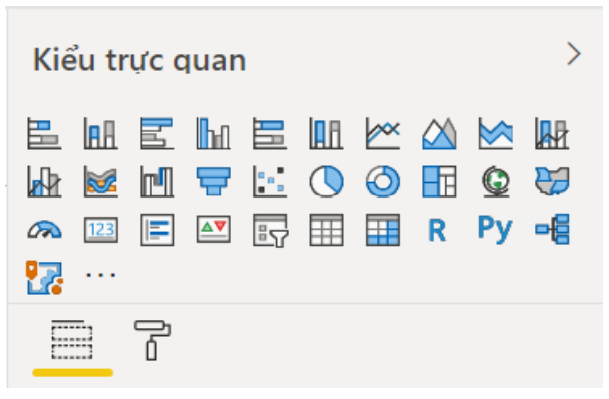
\includegraphics[scale = 1]{figures/Duyen/Các kiểu trực quan hóa dữ liệu trong PBI.PNG}
              \caption{Kết nối dữ liệu trong PBI}
            \end{figure}
\end{center}
Trực quan hóa dữ liệu là biểu diễn đồ họa của thông tin và dữ liệu. Bằng cách sử dụng các yếu tố trực quan như biểu đồ, đồ thị và bản đồ, các công cụ trực quan hóa dữ liệu cung cấp một cách dễ tiếp cận để xem và hiểu các xu hướng, ngoại lệ và mẫu trong dữ liệu.\\
Trong thế giới của Dữ liệu lớn, các công cụ và công nghệ trực quan hóa dữ liệu là rất cần thiết để phân tích một lượng lớn thông tin và đưa ra các quyết định dựa trên dữ liệu.\\
Trực quan hóa dữ liệu giúp bạn biến tất cả dữ liệu chi tiết đó thành thông tin kinh doanh dễ hiểu, hấp dẫn về mặt hình ảnh — và hữu ích.\\
Trực quan hóa dữ liệu làm cho dữ liệu trở nên sống động, khiến bạn trở thành người kể chuyện bậc thầy về những thông tin chi tiết ẩn trong các con số của bạn. Thông qua trang tổng quan trực tiếp, báo cáo tương tác, biểu đồ, đồ thị và các biểu thị trực quan khác, trực quan hóa dữ liệu giúp người dùng phát triển thông tin chi tiết mạnh mẽ về doanh nghiệp một cách nhanh chóng và hiệu quả.





\newpage
\section{Ứng dụng Data Warehouse và BI vào bài toán}
\subsection{Giới thiệu bài toán}
\subsubsection{Đặt vấn đề}
\textbf{Tổng quan về Health care: }\\
Health care hay chăm sóc sức khỏe là sự cải thiện sức khỏe thông qua phòng ngừa, chuẩn đoán, điều trị, cải thiện hoặc chữa bệnh, chấn thương và suy giảm thể chất và tinh thần khác ở người bệnh.\\

\textbf{Tổng quan về ảnh hưởng của thuốc lá đến phổi: }\\
Thuốc lá là nguyên nhân gây ra nhiều bệnh như: viêm họng, viêm phế quản, viêm phế quản phổi, bệnh phổi tắc nghẽn mạn tính, hen, ung thư phổi, ...\\
Bệnh phổi tắc nghẽn mạn tính là chỉ những tổn thương ở phổi có liên quan đến sự tắc nghẽn đường thở không phục hồi hoàn toàn. Mối liên quan giữa bệnh phổi tắc nghẽn mạn tính và hút thuốc cũng mạnh như với ung thư phổi.
Thuốc lá là nguyên nhân quan trọng nhất gây ra bệnh phổi tắc nghẽn mạn tính, có khoảng 15\% những người hút thuốc lá sẽ có triệu chứng lâm sàng của bệnh phổi tắc nghẽn mạn tính và 80 - 90\% người mắc bệnh phổi tắc nghẽn mạn tính là nghiện thuốc lá.\\
Ở hầu hết các nước, thuốc lá là nguyên nhân gây ra hơn 90\% ca tử vong vì ung thư phổi. Trung bình người hút thuốc làm tăng nguy cơ bị ung thư phổi lên từ 5 đến 10 lần so với người không hút thuốc.\\

\textbf{Lợi ích của kho dữ liệu đối với chăm sóc sức khỏe}
\begin{itemize}[label=$-$]
\item Báo cáo hiệu quả.
\item Quyết định lâm sàng tốt hơn.
\item Yêu cầu và thanh toán bảo hiểm được tối ưu hóa.
\item Cải thiện kinh nghiệm và kết quả của bệnh nhân.
\item Chăm sóc dựa trên giá trị được cá nhân hóa.
\item Lập kế hoạch chiến lược nâng cao.
\end{itemize}
\newpage
\subsubsection{Quy trình nghiệp vụ}
\begin{center}
            \begin{figure}[!h]
                \centering
                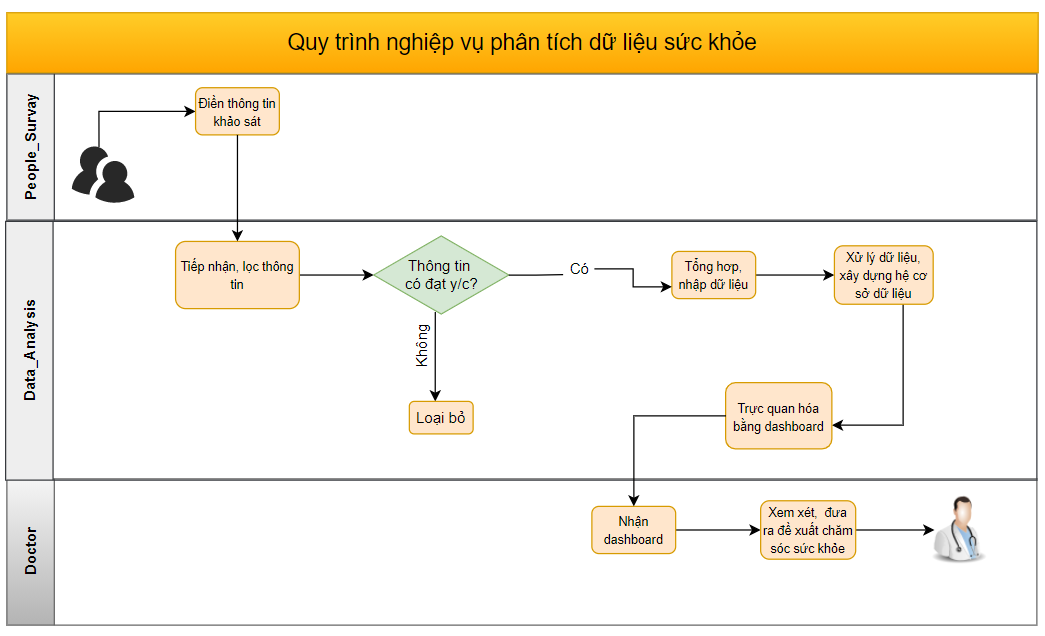
\includegraphics[scale = 0.6]{figures/Duyen/Phân tích nghiệp vụ.PNG}
              \caption{Quy trình nghiệp vụ}
            \end{figure}
\end{center}
%\newpage
\textbf{Quy trình xử lý}
\begin{itemize}[label=$-$]
    \item Đầu tiên, mọi người điền thông tin khảo sát.
    \item Sau đó, Data analysis sẽ tiến hành tiếp nhận và lọc thông tin, những thông tin không đạt yêu cầu sẽ bị loại bỏ ( Ví dụ những bản điền của người nào thiếu thông tin, thông tin điền không đúng ...), còn những thông tin đạt yêu cầu sẽ được tổng hợp, và xây dựng thành 1 bộ dữ liệu.
    \item Data analysis trực quan hóa bộ dữ liệu bằng dashboard và chuyển dashboard đến bác sĩ.
    \item Bác sĩ nhận dashboard, dựa vào đó để đưa ra những xem xét và đánh giá tình hình cũng như cách cải thiện sức khỏe của từng bệnh nhân.
\end{itemize}
\subsubsection{Quy mô dữ liệu}
Giới thiệu về bộ dữ liệu thì được chúng em lấy từ hệ thống giám sát yếu tố rủi ro hành vi là hệ thống điều tra qua điện thoại liên quan đến sức khỏe hàng đầu của quốc gia BRFSS.\\
Mục tiêu của hệ thống BRFSS: Thu thập dữ liệu tiểu bang về cư dân Hoa Kỳ về các hành vi nguy cơ liên quan đến sức khỏe, tình trạng sức khỏe mãn tính và việc sử dụng các dịch vụ phòng ngừa.\\
Kích thước bộ dữ liệu:
\begin{itemize}[label=$-$]
\newpage
    \item Dữ liệu gồm:
    \begin{itemize}[label=$+$]
        \item 3 file dữ liệu tương ứng với từng năm 2013 - 2015        \item Mỗi file chứa 1.5 triệu bản ghi.
    \end{itemize}
    \item Dữ liệu chủ yếu là dạng có cấu trúc
    \begin{itemize}
    \item Kích thước: 114MB
    \end{itemize}
    \item Chọn phân tích:
    \begin{itemize}[label=$+$]
        \item Dữ liệu khảo sát tại 6 tiểu bang: Alaska, California, Massachusetts, New York, Texas, Washington.
        \item 26 cột dữ liệu liên quan đến đối tượng khảo sát và vấn đề bệnh phổi mãn tính.
    \end{itemize}
\end{itemize}
%\newpage
\textbf{Mô tả 1 số trường dữ liệu quan trọng}
\begin{center}
            \begin{figure}[!h]
                \centering
                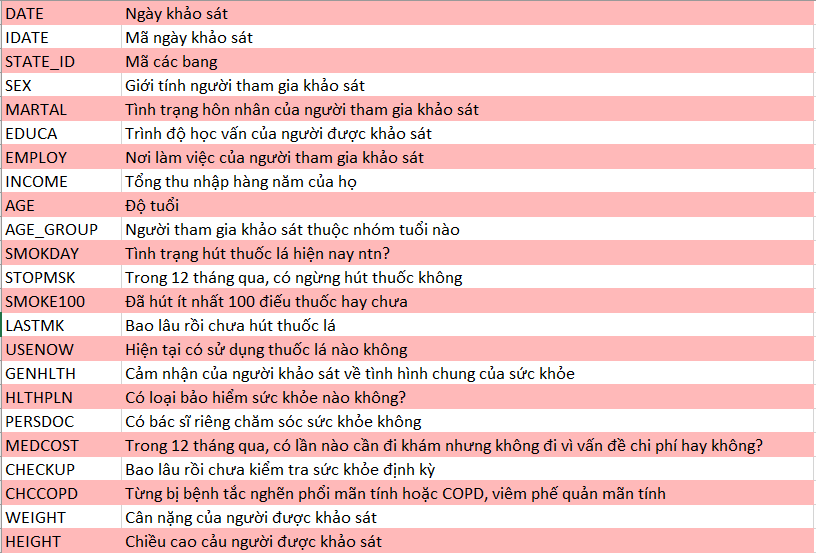
\includegraphics[scale = 1]{figures/Duyen/Mô tả 1 số trường dữ liệu quan trọng.PNG}
              \caption{Quy trình nghiệp vụ}
            \end{figure}
\end{center}
\subsubsection {Requirements}
\begin{itemize}
    \item \textbf{Input:} Dữ liệu khảo sát về ảnh hưởng của thuốc lá đối với phổi trong năm 2013 – 2015.
\item \textbf{Output: } Dashboard trả lời những câu hỏi:
\begin{enumerate}
    \item Phân tích và khảo sát thông tin người tham gia khảo sát:
    \begin{itemize}[label=$-$]
        \item Giới tính
        \item Độ tuổi
        \item Công việc
        \item Tình trạng hôn nhân
        \item Học vấn
        \item ...
    \end{itemize}
\item Phân tích và khảo sát tình trạng sức khỏe và khả năng tiếp cận y tế: 
    \begin{itemize}[label=$-$]
           \item  Tình trạng sức khỏe
            \item Có bảo hiểm y tế không?
            \item Có từng mắc bệnh phổi mãn tính không?
            \item Bao lâu chưa đi khám sức khỏe?    
            \item ...
        \end{itemize}
\item Phân tích và khảo sát thực trạng của việc hút thuốc lá:
    \begin{itemize}[label=$-$]
        \item Có hút thuốc lá không?
        \item Tần suất sử dụng thuốc lá?
        \item Đã từng hút ít nhất 100 điếu thuốc chưa?
        \item Đã từng có ý định bỏ thuốc lá chưa?
        \item ...
    \end{itemize}

\end{enumerate}
\end{itemize}




\newpage
\subsection{Phân tích và thiết kế hệ thống}

\subsubsection{Kiến trúc Dataware house}
\begin{enumerate}
    \item \textbf{Kiến trúc cũ:}
    \begin{center}
            \begin{figure}[!h]
                \centering
                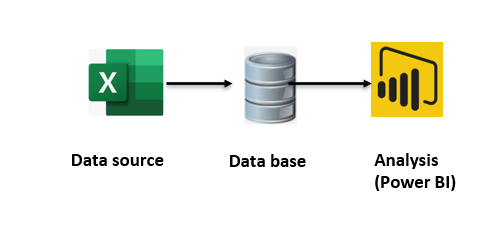
\includegraphics[scale = 1]{figures/Duyen/Kiến trúc cũ.PNG}
              \caption{Kiến trúc DW cũ}
            \end{figure}
\end{center}
    Mô hình cũ thực hiện các hoạt động phân tích dữ liệu ngay trên hệ thống lưu trữ. Điều này đem lại một số hạn chế như:
    \begin{itemize}[label=$-$]
        \item Làm giảm hiệu năng hệ thống 
\item Dữ liệu để phân tích không ổn định
\item Tốc độ xử lý chậm.
    \end{itemize}
Chính vì thế ta cần xây dựng mô hình mới để khắc phục được những hạn chế này:
    \item \textbf{ Kiến trúc mới:}\\
Đặc điểm hệ thống mới:
Sử dụng kiến trúc có vùng Staging, trong đó:
\begin{itemize}
    \item Nguồn dữ liệu là file CSV chứa dữ liệu thô.
    \item Vùng Staging là khu vực lưu trữ trung gian được sử dụng để thực hiện các bước ETL dữ liệu, ví dụ như xử lý dữ liệu Null, dữ liệu đa trị, định dạng kiểu dữ liệu, tách thành các bảng,...
    \item Data Warehouse là nơi dữ liệu được lưu trữ và quản lí để phục vụ cho việc phân tích thống kê, báo cáo, khai thác và trực quan hóa dữ liệu.
    \item Lớp phân tích được sử dụng để đưa ra các báo cáo và dashboard theo các chủ đề đã nêu thông qua một số công cụ trực quan hoá dữ liệu.
    
\end{itemize}\newpage
    \begin{center}
            \begin{figure}[!h]
                \centering
                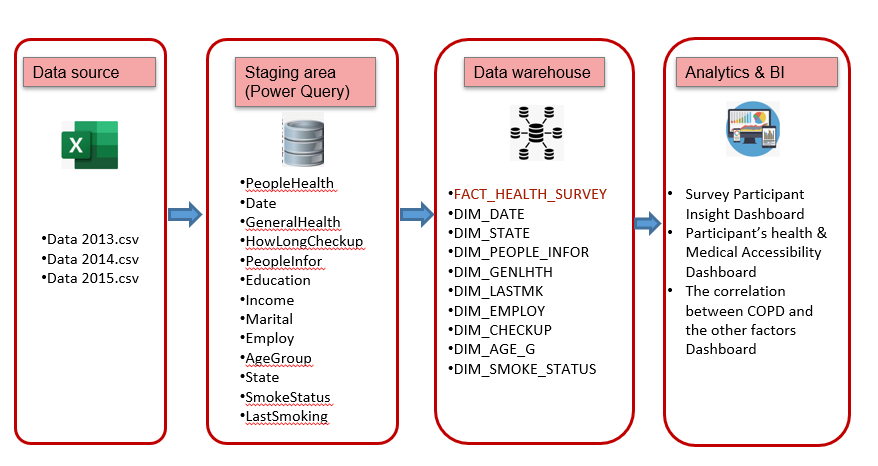
\includegraphics[scale = 0.8]{figures/Duyen/Kiến trúc mới.PNG}
              \caption{Kiến trúc DW mới}
            \end{figure}
\end{center}
\end{enumerate}

\newpage
\subsubsection{Data Exploration}
Thông tin của người thực hiện khảo sát
\begin{itemize}[label=$-$]
\item  Tỷ lệ giới tính 
\begin{center}
            \begin{figure}[!h]
                \centering
                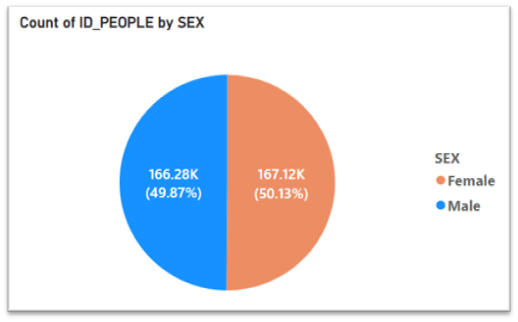
\includegraphics[scale = 0.8]{figures/Hoa/DE1.1.png}
              \caption{Tỷ lệ giới tính}
            \end{figure}
\end{center}
\begin{itemize}[label=$+$]
\item Từ biểu đồ ta thấy tỷ lệ giới tính của số người tham gia khảo sát là gần như ngang nhau : với tỷ lệ "Male" chiếm 49.78\% và tỷ lệ "Female" chiếm 50.13\%.
\end{itemize}

\item Độ tuổi tham gia khảo sát 
\begin{center}
            \begin{figure}[!h]
                \centering
                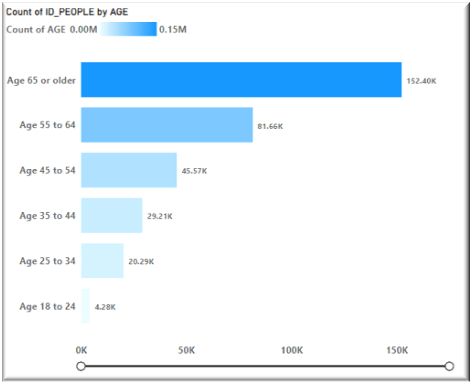
\includegraphics[scale = 0.8]{figures/Hoa/DE1.2.png}
              \caption{Độ tuổi tham gia khảo sát}
            \end{figure}
\end{center}
\begin{itemize}[label=$+$]
\item Ở khảo sát này thì có chia làm 6 nhóm tuổi và bắt đầu từ 18 tuổi trở lên.
\item Nhìn vào biểu đồ ta có thể thấy số lượng người tham gia khảo sát ở độ tuổi 65 tuổi trở lên rất cao lên đến 152.40K người, và số lượng người tham gia giảm dần theo chiều giảm của độ tuổi. Điều này cho thấy càng lớn tuổi con người càng có xu hướng quan tâm đến sức khỏe bản thân nhiều hơn.
\end{itemize}
\item Tình trạng việc làm 
\begin{center}
            \begin{figure}[!h]
                \centering
                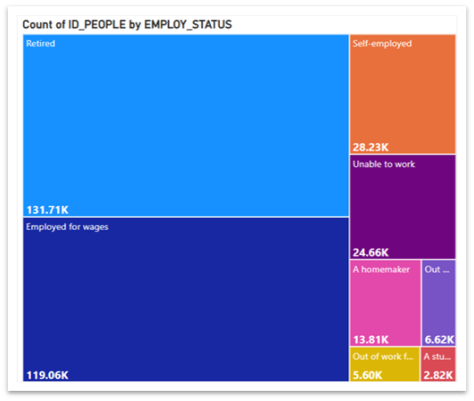
\includegraphics[scale = 0.8]{figures/Hoa/DE1.3.png} 
              \caption{Tình trạng việc làm }
            \end{figure}
\end{center}
\begin{itemize}[label=$+$]
\item Cũng tương tự như Độ tuổi tham gia khảo sát, có số lượng người từ 65 tuổi trở lên chiếm đa số thì tình trạng việc làm tương ứng là "Retired" ( Đã nghỉ hưu) cũng chiếm đa số, lên đến 131.71K người.
\item Số lượng người làm công ăn lương cũng chiếm một phần không nhỏ lên đến 119.06K người và ít nhất là học sinh, sinh viên.
\end{itemize}
\newpage
\item Tình trạng hôn nhân
\begin{center}
            \begin{figure}[!h]
                \centering
                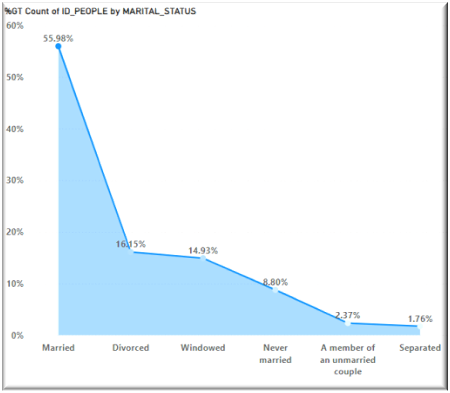
\includegraphics[scale = 0.7]{figures/Hoa/DE1.4.png} 
              \caption{Tình trạng hôn nhân }
            \end{figure}
\end{center}
\begin{itemize}[label=$+$]
\item Tình trạng hôn nhân của người tham gia khảo sát được chia thành 6 nhóm : Đã kết hôn, Đã ly hôn , Góa vợ hoặc chồng, Không bao giờ kết hôn, Chưa kết hôn, Ly thân.
\item Trong đó tỷ lệ người đã kết hôn chiếm đến 55.98\% điều đó cũng do hầu hết người được khảo sát từ 18 tuổi trở lên và phần lớn mọi người đã đủ khả năng để kết hôn.
\end{itemize}
\item Mức thu nhập
\begin{center}
            \begin{figure}[!h]
                \centering
                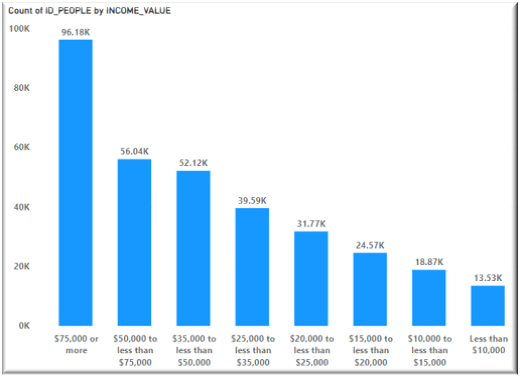
\includegraphics[scale = 0.7]{figures/Hoa/DE1.5.png} 
              \caption{Mức thu nhập }
            \end{figure}
\end{center}
\begin{itemize}[label=$+$]
\item Mức thu nhập được chia thành 8 nhóm trải dài từ ít hơn \$10.000 đến nhiều hơn \$75000.
\item Số người có mức thu nhất \$75.000 hoặc lớn hơn chiếm đa số lên đến 96.18K người, và giảm dần theo chiều giảm của mức thu nhập. Điều đó cho ta thấy phần lớn người tham gia khảo sát có thu nhập khá cao 
\end{itemize}
\end{itemize}
Khả năng tiếp cận y tế
\begin{itemize}[label=$-$]
\item Tỷ lệ người có bảo hiểm y tế
\begin{center}
            \begin{figure}[!h]
                \centering
                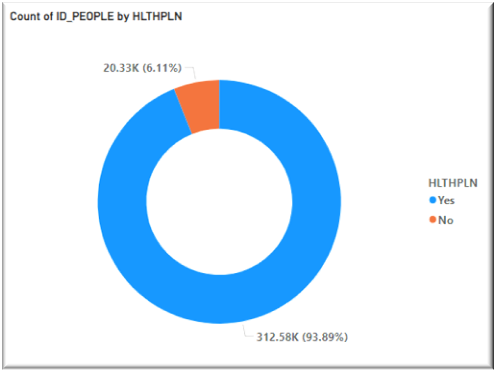
\includegraphics[scale = 0.9]{figures/Hoa/DE2.1.png} 
              \caption{Bảo hiểm y tế }
            \end{figure}
\end{center}
\begin{itemize}[label=$+$]
\item Số lượng người có bảo hiểm y tế lên đến 312.58K chiếm đến 93.89\%, điều này hoàn toàn phù hợp với mức thu nhập cao của số người tham gia khảo sát.
\item Tuy nhiên vẫn còn đến 20.33K người chưa có bảo hiểm y tế, cho thấy khả năng tiếp cận y tế của họ vẫn chưa cao.
\end{itemize}\newpage
\item Tỷ lệ giữa các khoảng thời gian chưa đi kiểm tra sức khỏe theo từng  khu vực
\begin{center}
            \begin{figure}[!h]
                \centering
                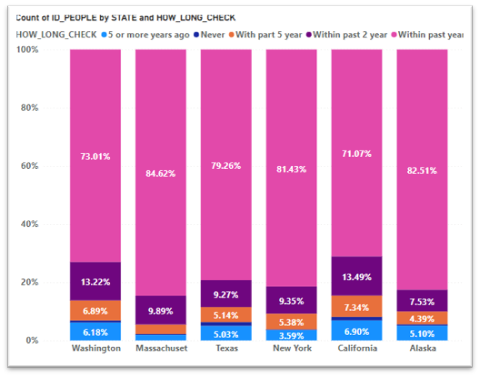
\includegraphics[scale = 0.8]{figures/Hoa/DE2.2.png} 
              \caption{Thời gian đi kiểm tra sức khỏe }
            \end{figure}
\end{center}
\begin{itemize}[label=$+$]
\item Thời gian đi kiểm tra sức khỏe được chia làm 4 nhóm theo độ dài của thời gian.
\item Ta có thể thấy phần lớn mọi người đi kiểm tra sức khỏe trước đó chưa đến 1 năm 
\item Bên cạnh đó vẫn có nhiều người khám sức khỏe trước đó 2 năm, 5 năm và thậm chí là nhiều hơn 5 năm.
\end{itemize}
\item Số người có bác sĩ riêng theo từng khu vực
\begin{center}
            \begin{figure}[!h]
                \centering
                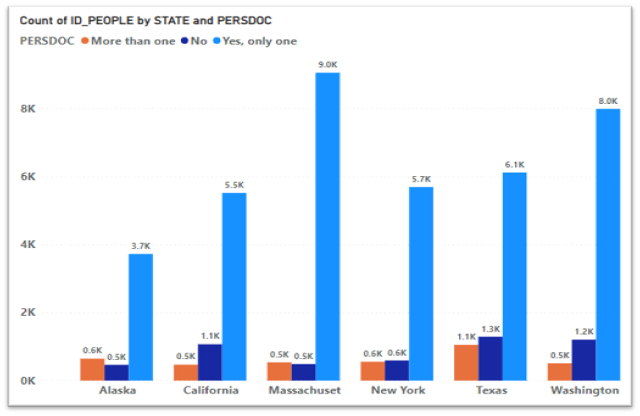
\includegraphics[scale = 0.6]{figures/Hoa/DE2.3.png} 
              \caption{Bác sĩ riêng }
            \end{figure}
\end{center}
\begin{itemize}[label=$+$]
\item Nhìn vào báo cáo ta có thể thấy, phần lớn người tham gia khảo sat có 1 bác sĩ riêng, và cũng có một phần người có nhiều hơn 1 bác sĩ riêng.
\item Có một phần người tham gia khảo sát không có bác sĩ riêng, họ là những người có mức thu nhập thấp và có khả năng tiếp cận y tế thấp.
\end{itemize}
\end{itemize}
Thực trạng của việc hút thuốc lá
\begin{itemize}[label=$-$]
\item Số người sử dụng thuốc lá theo từng nhóm tuổi
\begin{center}
            \begin{figure}[!h]
                \centering
                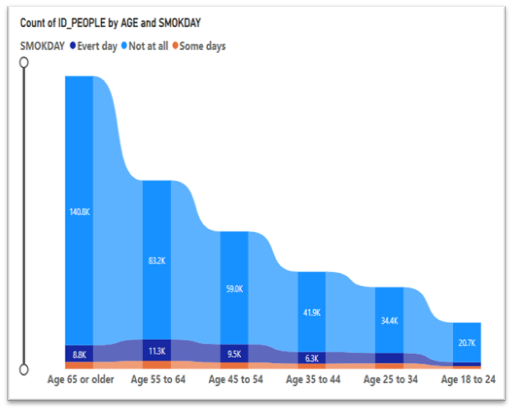
\includegraphics[scale = 0.9]{figures/Hoa/DE3.1.png} 
              \caption{Theo độ tuổi }
            \end{figure}
\end{center}
\begin{itemize}[label=$+$]
\item Biểu đồ cho thấy phần lớn người tham gia khảo sát không hút thuốc lá
\item Nhưng vẫn có một bộ phận người hút thuốc lá hàng ngày và cao nhất ở nhóm tuổi từ 55 đến 64.
\end{itemize}\newpage
\item Tình trạng hút thuốc lá ở từng khu vực 
\begin{center}
            \begin{figure}[!h]
                \centering
                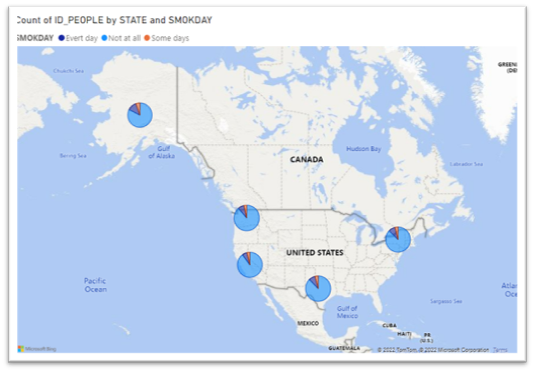
\includegraphics[scale = 0.9]{figures/Hoa/DE3.2.png} 
              \caption{Theo khu vực }
            \end{figure}
\end{center}
\begin{itemize}[label=$+$]
\item Tỉ lệ hút thuốc lá ở các khu vực là gần như nhau, phần lớn mọi người đều không sử dụng thuốc lá.
\end{itemize}
\end{itemize}\newpage

\subsubsection{ETL}

Dữ liệu gốc chứa gần 1,5 triệu bản ghi các dữ liệu đều đã được mã hóa dưới dạng số. Tha thực hiện ETL dữ liệu bằng Excel  gồm các thao tác như thay thế giá trị , đổi kiểu dữ liệu , tách cột , xử lý các cột ngày tháng 
Đầu tiên đưa dữ liệu vào Power query .Nhận thấy có 3 file dữ liệu của năm 2013 , 2014, 2015 đều có các cột tương ứng giống nhau . Để giúp cho việc thống kê và báo cáo được dễ dàng hơn  ta thực hiện nối các bảng lại với nhau bằng cách sử dụng \textit{Append Quieries } .\\
\\\textbf{Xử lý dữ liệu mã hóa }\\
Các dữ liệu trong bảng 2013, 2014,2015 đều đã được mã hóa dưới dạng số. Do đó cần phải giải mã chúng để đưa về các giá trị cụ thể chi tiết hơn. Có rất nhiều cách để giải mã như tách cột, thêm cột, thêm cột có
điều kiện, thay thế giá trị, .... Cụ thể:
\begin{itemize}
    \item Giải mã dữ liệu cột IDAY , IMONTH , IYEAR \\\hfill
    Nhận thấy dữ liệu trong các cột \textit{IDAY, IMONTH ,IYEAR} đều được bao bọc bởi cặp dấu \textbf{''} do đó cần phải tách dữ liệu ra bằng cách xử dụng \textit{Split Column } với dấu phân cách là \textbf{'}. Ta thu được kết quả khi tách cột \textit{IMONTH} như hình dưới :\\
    
            \begin{figure}[!h]
                \begin{center}
                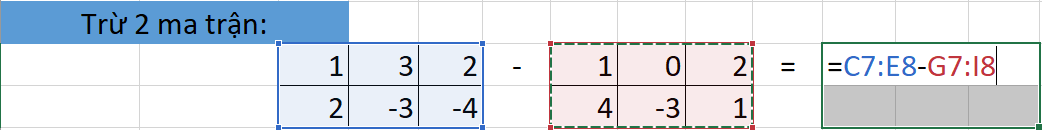
\includegraphics[scale = 0.8]{HONG/2.png}
              \caption{Tách dữ liệu cột IMONTH}
         
\end{center}
   \end{figure}
   Sau khi đã tách dữ liệu của 3 cột ta thực hiện xóa các cột \texit{IMONTH.1,IMONTH.3 , IYEAR.1 ,IYEAR.3 ,IDAY.1 ,IDAY.3 }bởi vì các cột này đều không có giá trị sử dụng . Thực hiện gộp các cột \textit{ IDAY.2 , IMONTH.2 ,IYEAR.2  }  với nhau bằng cách sử dụng\textit{ merge columns} với seperator là / , sau đó chuyển dữ liệu về dạng ngày tháng ta thu được kết quả như hình dưới đây :
    \begin{figure}[!h]
                \begin{center}
                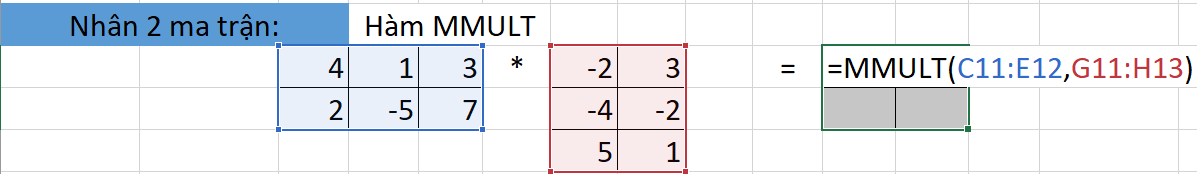
\includegraphics[scale = 0.8]{HONG/3.png}
              \caption{Merge quieres}
         
\end{center}
   \end{figure}
   \item Giải mã hóa các cột giá trị khác \\\hfill
   Thực hiện thay thế các giá trị số thành các giá trị cụ thể ví dụ như ở cột \textbf{SEX} chỉ có 2 giá trị số là 1 và 2 , nhìn vào giá trị ta không thể biết được nó có nghĩa là gì do đó ta cần giải mã nó với 1 tương ứng là\textit{ male} , với 2 tương ứng là\textit{ female }.
   Thực hiện giải mã bằng cách thay thế giá trị (sử dụng replace values ) hoặc megre quieres bảng gốc với bảng dữ liệu giải mã tương ứng . Tuy nhiên khi dữ liệu bị mã hóa có nhiều việc thay thế giá trị sẽ rất là tốn thời gian do đó ta thực hiện merge quieres thu được kết quả như hình dưới
     \begin{figure}[!h]
                \begin{center}
                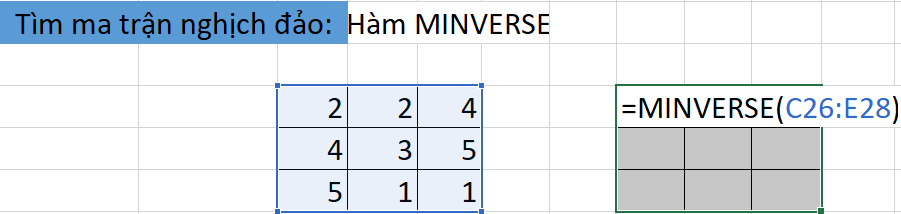
\includegraphics[scale = 0.8]{HONG/5.png}
                \caption{Merge quieres}
                \end{center}
    \end{figure}
\end{itemize}
\textbf{Xóa các giá trị \textit{NULL} trong bảng }\\
Thực hiện xóa các giá trị \textit{NULL} ở mỗi bảng .Các giá trị này sẽ làm cho việc báo cáo thống kê phức  tạp do đó ta cần thực thao tác xóa . Dưới đây là kết quả của quá trình xóa các giá trị null trong cột \textbf{LASTSMK2} :
 
            \begin{figure}[!h]
                \begin{center}
                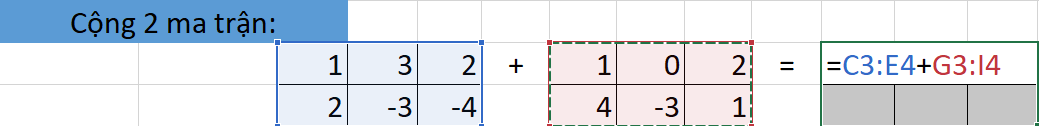
\includegraphics[scale = 0.7]{HONG/1.png}
              \caption{Xóa giá trị NULL cột LASTSMK2}
         
\end{center}
   \end{figure}


Ngoài ra để tiện cho việc truy vấn dữ liệu  ta có thể lưu dữ liệu vào cơ sở dữ liệu:\\
\begin{itemize}
    \item Dữ liệu sau khi được xử lí đơn giản được lưu vào CSDL HealthCare, vùng dữ liệu
được lưu này gọi là Stagging, là vùng đệm chứa dữ liệu trước khi đưa vào kho dữ liệu.
\item Xây dựng kho dữ liệu bằng cách tạo các bảng trong cơ sở dữ liệu theo mô hình OLAP
đã được thiết kế.

\end{itemize}
Đổ dữ liệu từ cơ sở dữ liệu vào kho dữ liệu bằng cách sử dụng SQL Server Import and Export Wizard trong SQL sever:\newpage
\begin{center}
            \begin{figure}[!h]
                \centering
                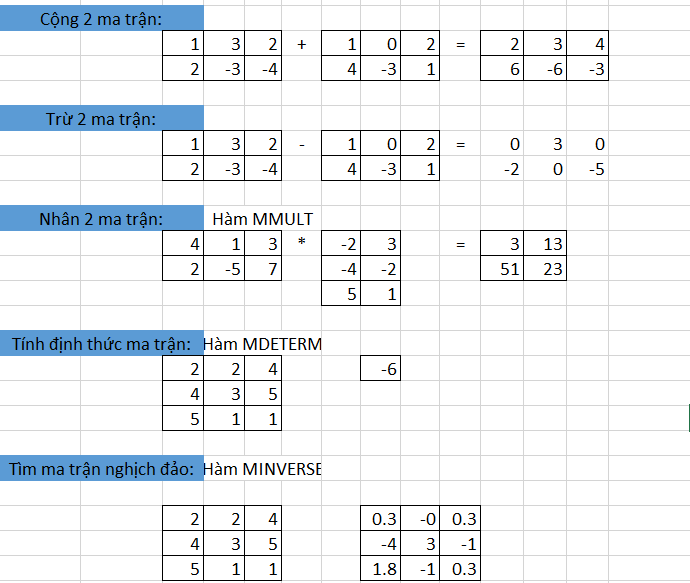
\includegraphics[scale = 0.9]{HONG/6.png} 
              \caption{IMPORT DATA}
            \end{figure}
\end{center}
\begin{itemize}
    \item Các dữ liệu cố định, không thay đổi theo thời gian sẽ được chuyển trực tiếp từ Stagging vào Kho dữ liệu thông qua câu lệnh “Insert” như bên dưới :
    \begin{center}
            \begin{figure}[!h]
                \centering
                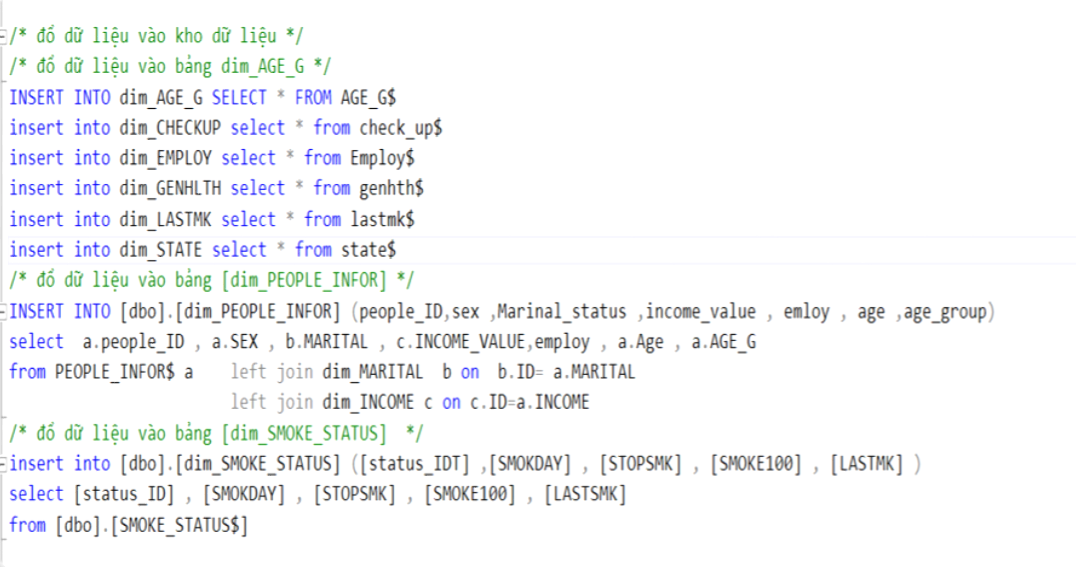
\includegraphics[scale = 0.6]{HONG/8.png} 
              \caption{Câu lệnh INSERT}
            \end{figure}
\end{center}
\item Đối với các dữ liệu được cập nhật định kì theo thời gian (tức là cứ sau một khoảngthời gian sẽ có dữ liệu) mới được thêm vào thì việc cứ mỗi lần  phải viết lại câu lệnh “Insert” là rất mất thời gian. Thay vào đó, ta sẽ đưa câu lệnh “Insert” tạo thành một thủ tục để mỗi lần cập nhật dữ liệu ta chỉ cần gọi thủ thục một cách nhanh chóng:
\begin{center}
            \begin{figure}[!h]
                \centering
                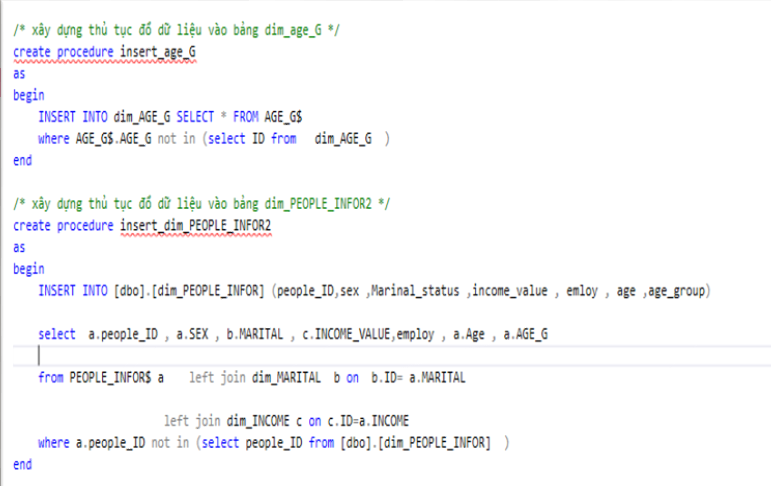
\includegraphics[scale = 0.75]{HONG/9.png} 
              \caption{Thủ tục INSERT}
            \end{figure}
\end{center}
Sau khi đã xây dựng xong các thủ tục ta thử kiểm tra lại kết quả :
\begin{center}
            \begin{figure}[!h]
                \centering
                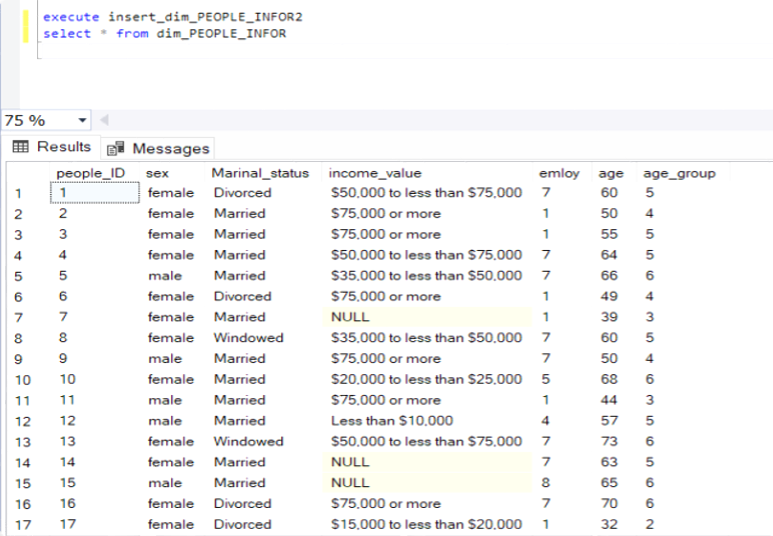
\includegraphics[scale = 0.75]{HONG/10.png} 
              \caption{Kết quả}
            \end{figure}
\end{center}
\end{itemize}
\newpage
\subsubsection{Facts}
Chủ điểm phân tích của hệ thống được mô tả trong bảng "FACT\_HEALTH\_SURVEY" với khoá chính là SURVEY\_ID và 4 khoá phụ bao gồm: PEOPLE\_ID, REGION\_ID, DATE\_ID, STATUS\_ID cùng với thuộc tính CHCCOPD.
\begin{center}
            \begin{figure}[!h]
                \centering
                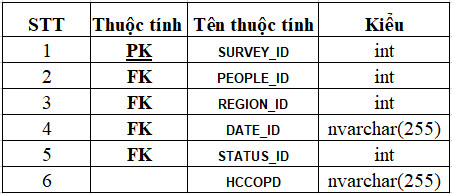
\includegraphics[scale = 0.9]{van/fact.png} 
              \caption{FACT\_HEALTH\_SURVEY}
            \end{figure}
\end{center}

\subsubsection{Dimension}
Theo chủ điểm phân tích FACT\_HEALTH\_SURVEY" ta có các chiều phân tích theo thời gian, tính trạng sức khoẻ, thông tin của người tham gia khảo sát, tình trạng hút thuốc và khu vực.
\begin{itemize}
    \item Chiều về thời gian\\
    Chiều về thời gian bao gồm thời gian tham gia khảo sát với khoá chính là DATE\_ID.
    \begin{center}
            \begin{figure}[!h]
                \centering
                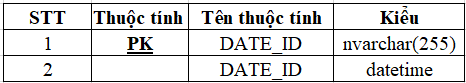
\includegraphics[scale = 0.8]{van/dim_date.jpg}
              \caption{OLAP DIM\_DATE}
            \end{figure}
    \end{center}
    \item Chiều về tình trạng sức khoẻ của người tham gia khảo sát\\
    Có khoá chính là PEOPLE\_ID và 7 thuộc tính lần lượt là: HEALTH\_STATUS, HLTHPLN, PERSDOC, MEDCOST, HOW\_LONG\_CHECKUP, WEIGHT\_KG, HEIGHT\_CM.
    \begin{center}
            \begin{figure}[!h]
                \centering
                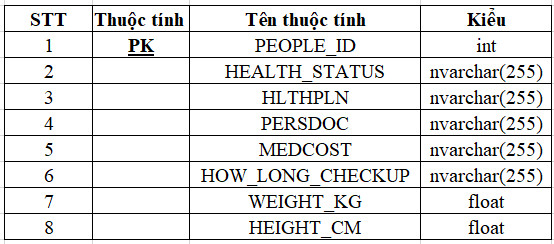
\includegraphics[scale = 0.8]{van/oltp dim heath.png}
              \caption{OLAP DIM\_HEALTH}
            \end{figure}
    \end{center}
    \item Chiều về thông tin người tham gia khảo sát\\
    Được phân cấp thành 3 bảng như sau:
    \begin{center}
            \begin{figure}[!h]
                \centering
                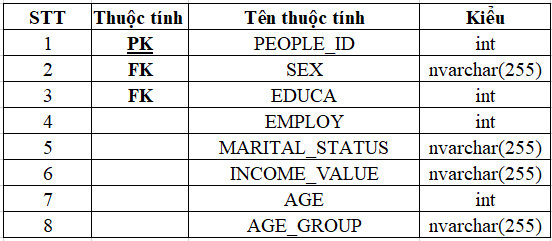
\includegraphics[scale = 0.8]{van/olap dim people infor.png}
              \caption{OLAP DIM\_PEOPLE\_INFOR}
            \end{figure}
    \end{center}
    \begin{center}
            \begin{figure}[!h]
                \centering
                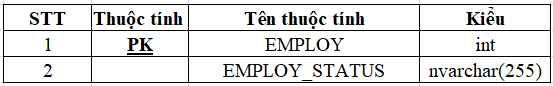
\includegraphics[scale = 0.8]{van/olap dim employ.jpg}
              \caption{OLAP DIM\_EMPLOY}
            \end{figure}
    \end{center}
    \begin{center}
            \begin{figure}[!h]
                \centering
                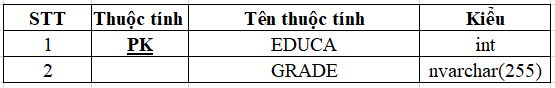
\includegraphics[scale = 0.8]{van/olap dim education.jpg}
              \caption{OLAP DIM\_EDUCATION}
            \end{figure}
    \end{center}
    \item Chiều về tình trạng hút thuốc của người tham gia khảo sát\\
    Gồm một khoá chính STATUS\_ID và 5 thuộc tính: SMOKEDAY, STOPSMK, SMOKE100, HOW\_LONG\_LAST\_SMOKE, USENOW.
    \begin{center}
            \begin{figure}[!h]
                \centering
                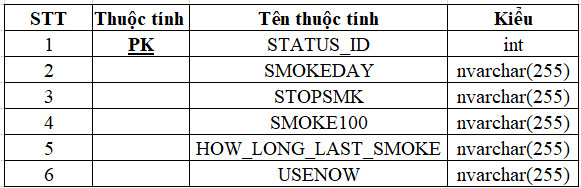
\includegraphics[scale = 0.8]{van/olap dim smoke status.png}
              \caption{OLAP DIM\_SMOKE\_STATUS}
            \end{figure}
    \end{center}
    \item Chiều về địa điểm khu vực khảo sát\\
    Gồm một khoá chính REGION\_ID và thuộc tính STATE.
    \begin{center}
            \begin{figure}[!h]
                \centering
                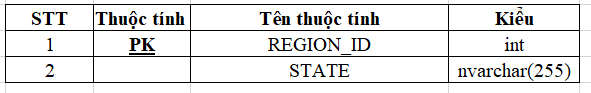
\includegraphics[scale = 0.8]{van/olap dim region.png}
              \caption{OLAP DIM\_SMOKE\_STATUS}
            \end{figure}
    \end{center}
\end{itemize}
\newpage
Sau đây là phần thống kê dữ liệu theo các chiều:
\begin{itemize}
    \item Chiều về thời gian
    \begin{center}
            \begin{figure}[!h]
                \centering
                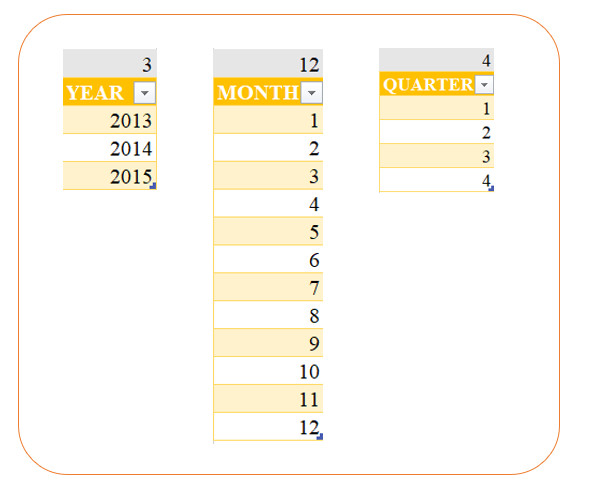
\includegraphics[scale = 0.6]{van/dim_tg.png}
              %\caption{OLAP DIM\_SMOKE\_STATUS}
            \end{figure}
    \end{center}
    \item Chiều về tình trạng sức khoẻ người tham gia khảo sát
    \begin{center}
            \begin{figure}[!h]
                \centering
                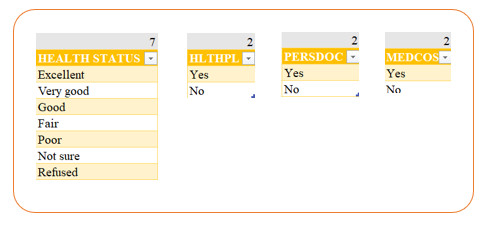
\includegraphics[scale = 0.6]{van/dim_sk.png}
              %\caption{OLAP DIM\_SMOKE\_STATUS}
            \end{figure}
    \end{center}
    \newpage 
    \item Chiều về khu vực
    \begin{center}
            \begin{figure}[!h]
                \centering
                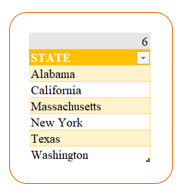
\includegraphics[scale = 0.6]{van/dim_kv.png}
              %\caption{OLAP DIM\_SMOKE\_STATUS}
            \end{figure}
    \end{center} 
    \item Chiều về tình trạng hút thuốc của người tham gia khảo sát 
    \begin{center}
            \begin{figure}[!h]
                \centering
                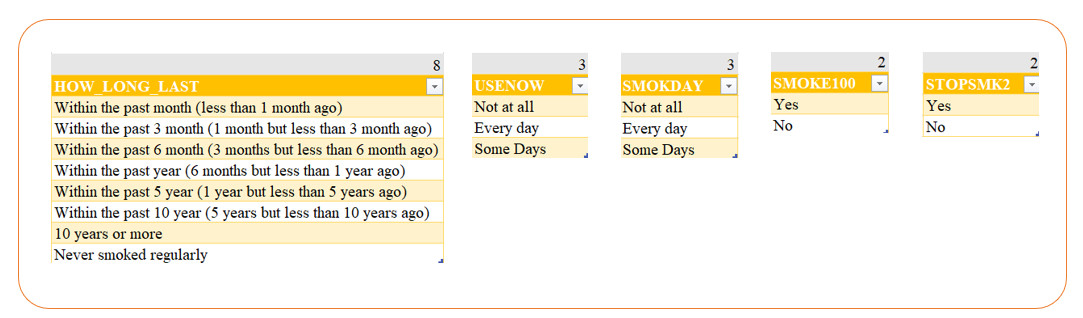
\includegraphics[scale = 0.4]{van/dim_tt.png}
              %\caption{OLAP DIM\_SMOKE\_STATUS}
            \end{figure}
    \end{center}
    \item Chiều về thông tin người tham gia khảo sát
    \begin{center}
            \begin{figure}[!h]
                \centering
                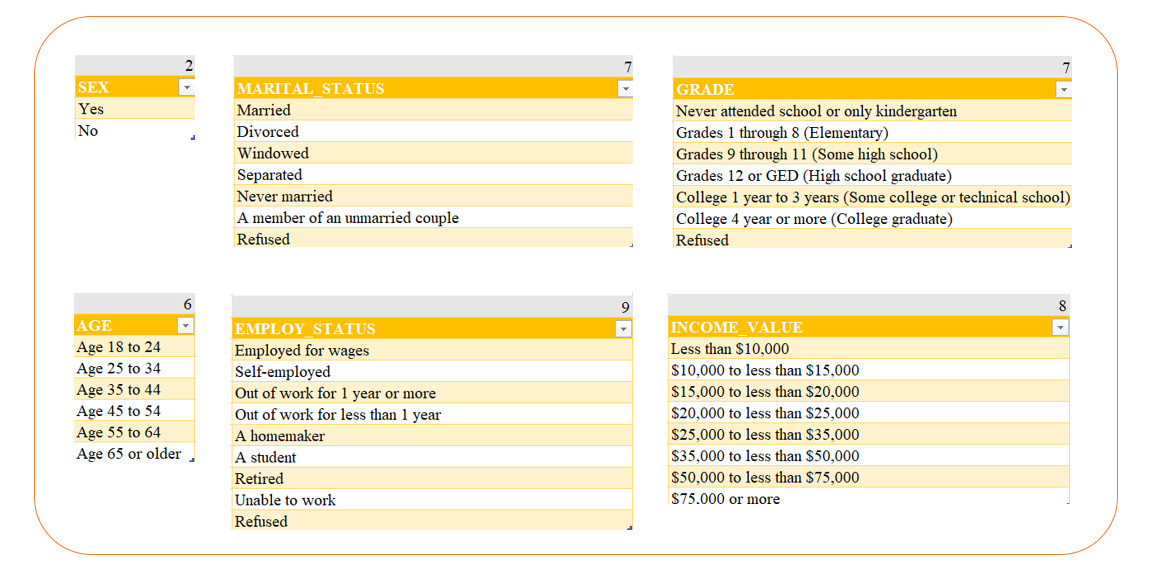
\includegraphics[scale = 0.4]{van/dim_inf.png}
              %\caption{OLAP DIM\_SMOKE\_STATUS}
            \end{figure}
    \end{center}
    
\end{itemize}

\subsubsection{Data model-ERD}
\begin{center}
            \begin{figure}[!h]
                \centering
                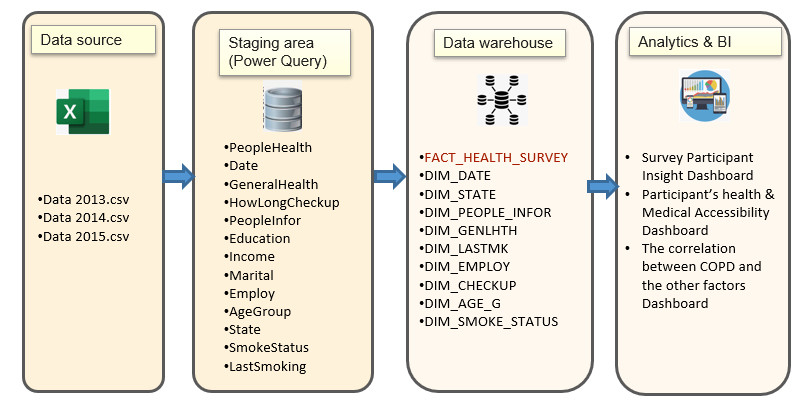
\includegraphics[scale = 0.4]{van/oltp healthcare.png}
              \caption{Kiến trúc hệ thống OLAP Healthcare}
            \end{figure}
    \end{center}
    Tầng dưới cùng là hệ CSDL quan hệ “DataCo\_OLTP”. Các công cụ đầu cuối, các tiện ích được dùng để đưa dữ liệu vào tầng dưới cùng từ hệ cơ sở dữ liệu hoạt động hoặc từ nguồn bên ngoài (file csv, excel...). Những công cụ và tiện ích này thực hiện việc loạibỏ dữ liệu thừa, làm sạch dữ liệu, chuyển đổi dữ liệu, cập nhật dữ liệu. Dữ liệu được lưu trữ vào 13 bảng: 
    
\begin{itemize}
    \item PEOPLEHEALTH
    \item DATE
    \item GENARALHEALTH
    \item HOWLONGCHECKUP
    \item PEOPLEINFOR
    \item EDUCATION
    \item INCOME
    \item MARITAL
    \item EMPLOY
    \item AGEGROUP
    \item STATE
    \item SMOKESTATUS
    \item LASTSMOKING
\end{itemize}

Tầng giữa là Data warehouse “DataCo\_OLAP” được cài đặt dùng mô hình quan hệ OLAP. Dữ liệu được đổ từ mô hình OLTP của hệ CSDL hoạt động sang mô hình OLAP của Data warehouse, bao gồm các bảng:
\begin{itemize}
    \item FACT\_HEALTH\_SURVEY
    \item DIM\_HEALTH
    \item DIM\_DATE
    \item DIM\_REGION
    \item DIM\_PEOPLE\_INFOR
    \item DIM\_EDUCATION
    \item DIM\_EMPLOY
    \item DIM\_SMOKE\_STATUS
\end{itemize}
Tầng trên cùng là tầng người dùng cuối, gồm các câu truy vấn và các công cụ làm báo cáo, phân tích, công cụ khai thác dữ liệu về:
\begin{itemize}
    \item Survey Participant Insight Dashboard: thông tin chi tiết người tham gia khảo sát.
    \item Participant’s health \& Medical Accessibility Dashboard: tổng quan về khả năng tiếp cập y tế và sức khỏe người tham gia khảo sát.
    \item The correlation between COPD and the other factors Dashboard: mối tương quan giữa COPD và các yếu tố khác.
\end{itemize}
\newpage
\subsubsection{Data model OLAP}
Mô hình logic
\begin{center}
        \begin{figure}[!h]
            \centering
            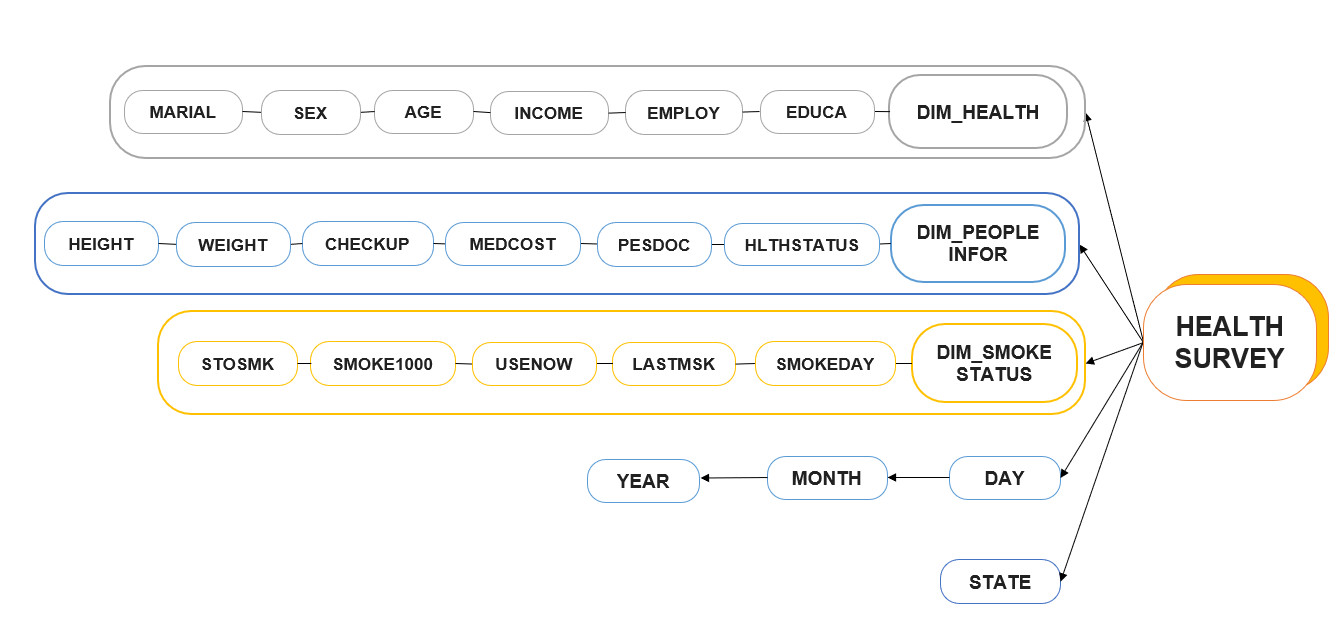
\includegraphics[scale = 0.35]{van/oltp_logic.png}
             \caption{Mô hình logic của hệ thống OLAP}
        \end{figure}
\end{center}

Mô hình quan hệ
\begin{center}
        \begin{figure}[!h]
            \centering
            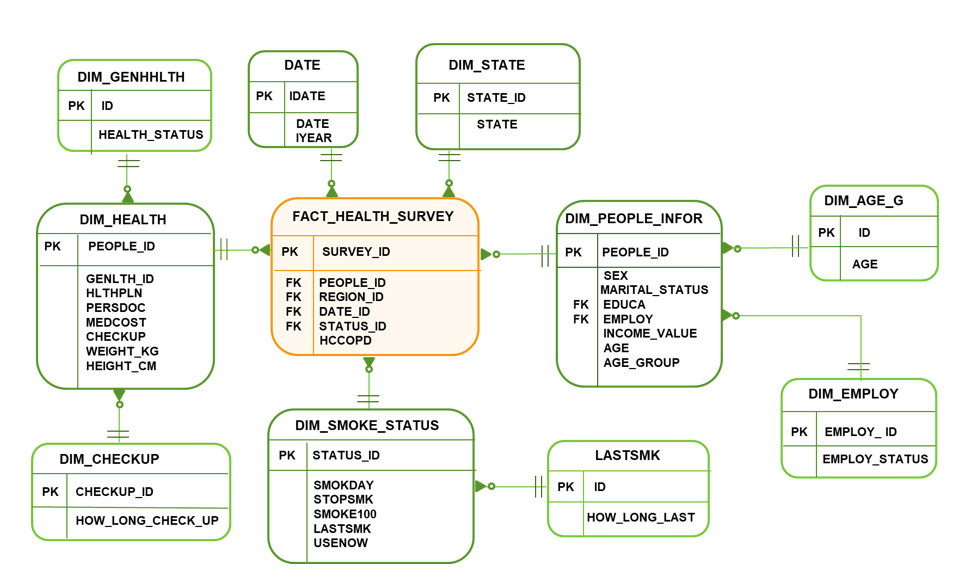
\includegraphics[scale = 0.4]{van/oltp_erd.png}
             \caption{Mô hình quan hệ của hệ thống OLAP}
        \end{figure}
\end{center}
    








\newpage
\subsection{Xây dựng hệ thống}

\subsubsection{Xây dựng Dashboard}
\begin{enumerate}
    \item \textbf{Khảo sát thông tin của những người tham gia thực hiện khảo sát}\\
    Dashboard thể hiện tổng quan nhất về những người tham gia thực hiện khảo sát này với các yếu tố như độ tuổi, giới tính, trình độ học vấn, thu nhập,... thông qua
    \begin{itemize}[label=$-$]
        \item Cart thể hiện tổng số người tham gia và tất cả các khu vực.
        \item Slicer theo các thuộc tính age, state, year, fmonth để có thể linh hoạt lọc ra các thông tin theo mong muốn.
        \item Một số biểu đồ như Pie chart, Donut chart, map, treemap,...
    \end{itemize}
    \begin{center}
        \begin{figure}[!h]
            \centering
            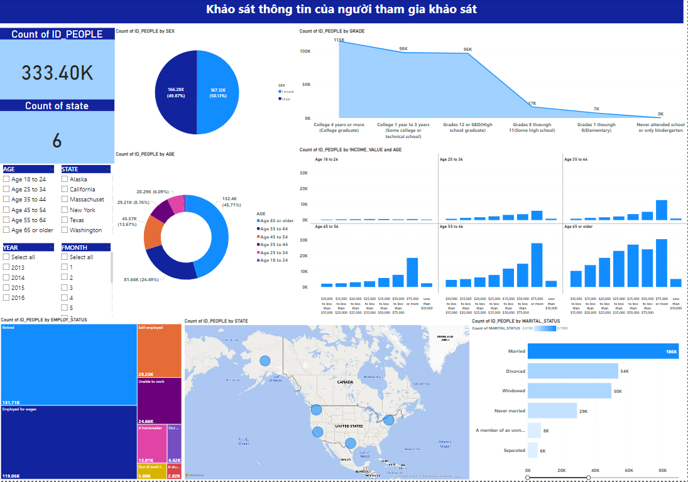
\includegraphics[scale = 0.8]{trang/dashboard1.png}
          \caption{Khảo sát thông tin của những người tham gia thực hiện khảo sát}
        \end{figure}
    \end{center}
    Từ Dashboard này ta có được thông tin phân tích như sau
    \begin{itemize}[label = $-$]
        \item Có tổng cộng tất cả là 333.4 nghìn người tham gia thực hiện khảo sát đến từ 6 bang được phân thành 6 nhóm tuổi chính từ 18 đến 24 tuổi, từ 25 đến 34 tuổi, từ 35 đến 44, từ 45 đến 54, từ 55 đến 64 tuổi và từ 65 tuổi trở lên.
        
        \item Về giới tính của người tham gia khảo sát thì tỷ lệ giữa nam và nữ là xấp xỉ nhau với nữ là 50,13\% và nam là 49,87\%.
        
        \item Về độ tuổi thì ta thấy nhóm tuổi tham gia thực hiện nhiều nhất là từ 65 tuổi trở lên chiếm 45,71\% trên tổng tất cả các nhóm tuổi, tiếp đến là nhóm từ 55 đến 64 tuổi chiếm 24,49\% và tỷ lệ này có xu hướng giảm dần theo độ tuổi, thấp nhất là nhóm từ 18 đến 24 tuổi với 1,28\%.
        
        \item Về trình độ học vấn thì số người đã tốt nghiệp cao đẳng,đại học đa số chiếm phần lớn và xếp sa lần lượt là đang học cao đẳng, đại học và tốt nghiệp lớp 12.
        
        \item Về thu nhập thì ở nhóm tuổi từ 18 đến 24 tuổi mức thu nhập được trải đều còn với các nhóm tuổi còn lại thì mức thu nhập hầu hết là hơn \$ 75000, riêng với nhóm từ 65 tuổi trở lên thì tỷ lệ mức thu nhập từ dưới \$ 75000 nhiều hơn so với các bảng còn lại.
        
        \item Về tình trạng việc làm vì chủ yếu người tham gia khảo sát là trên 65 tuổi nên đa số đã về hưu, theo sau đó là những người làm công ăn lương cũng chiếm khá đông.
        
        \item Về số lượng người tham gia thực hiện theo vị trí địa lý ta thấy tỷ lệ người tham gia từ các bang là tương đương nhau.
        
        \item Về tình trạng hôn nhân thì chủ yếu là những người đã kết hôn với hơn 186 nghìn người trên tổng số hơn 333 nghìn người chiếm hơn 50\%.
    \end{itemize}
Qua đó, ta thấy khảo sát này được thực hiện đa số ở những người trung tuổi nên hầu hết đã có việc làm hoặc đã về hưu và tuy họ ở các khu vực khác nhau nhưng đời sống đều ở mức ổn định.
    
    \item \textbf{Khảo sát về khả năng tiếp cận y tế}\\
    Khả năng tiếp cận y tế tùy thuộc vào hoàn cảnh của mỗi người nên việc xây dựng Dashboard này để thể hiện các vấn đề về việc khám sức khỏe với 
    \begin{itemize}[label=$-$]
        \item Cart thể hiện tổng số người tham gia và tất cả các khu vực.
        \item Slicer theo các thuộc tính age, state, year, fmonth để có thể linh hoạt lọc ra các thông tin theo mong muốn.
        \item Một số biểu đồ như Pie chart, Donut chart, Area chart, 100\% Stacked column chart,...
    \end{itemize}
    \begin{center}
            \begin{figure}[!h]
                \centering
                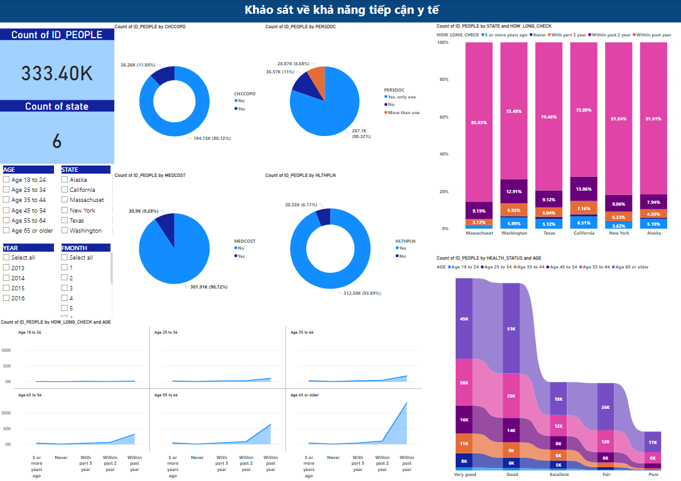
\includegraphics[scale = 0.8]{trang/dashboad2.png}
              \caption{Khảo sát về khả năng tiếp cận y tế}
            \end{figure}
\end{center}
    \newpage
    Từ Dashboard này ta có được thông tin phân tích như sau
    \begin{itemize}[label=$-$]
        \item Tỷ lệ người từng mắc bệnh tắc nghẽn phổi mãn tính là 11,88\%.
        
        \item Số người có bác sĩ riêng chiếm khá ca trong đó có đến 80,32\% là có một bác sĩ riêng và 8,68\% là nhiều hơn một bác sĩ.
        
        \item Trong đó cũng có những người chưa có đủ điều kiện đi thăm khám bác sĩ cần thiết trong vòng 12 tháng qua chiếm 9,28\%.
        
        \item Số người tham gia bảo hiểm y tế rất cao chiếm gần 94\%.
        
        \item Về lần cuối đi khám sức khỏe, ta thấy mọi người thường xuyên đi khám sức khỏe và nhóm từ 65 tuổi trở lên có tỷ lệ đi khám sức khỏe lớn nhất do càng lớn tuổi thì sẽ càng quan tâm chăm sóc sức khỏe nhiều hơn, ngược lại nhóm từ 18 đến 24 tuổi chiếm tỷ lệ thấp nhất.
        
        \item Xét về từng khu vực thì thấy Massachuset có tỷ lệ thăm khám đều đặn hơn so với các khu vực còn lại.
        
        \item Về tình trạng sức khỏe theo độ tuổi thì từ 18 đến 24 tuổi trạng thái tốt hơn hẳn, từ 25 đến 64 tuổi có sức khỏe tốt chiếm phần lớn và trên 65 tuổi trở lên số người có tình trạng không ổn chiếm nhiều hơn so với các nhóm tuổi khác, đó cũng là điều dễ hiểu.
    \end{itemize}
 Qua đó, ta thấy về chất lượng cuộc của những người này khá ổn với đa số người có bác sĩ riêng và có tham gia bảo hiểm y tế, về việc đi khám sức khỏe cũng được diễn ra thường xuyên.
    
    \item \textbf{Khảo sát về tình trạng hút thuốc lá}\\
    Dashboard thể hiện tình trạng hút thuốc lá theo các yếu tố như độ tuổi, tần suất sử dụng,...  
    \begin{itemize}[label=$-$]
        \item Slicer theo các thuộc tính age, state, fmonth để có thể linh hoạt lọc ra các thông tin theo mong muốn.
        \item Một số biểu đồ như Pie chart, Donut chart, Area chart, Clustered column chart,...
    \end{itemize}
    \begin{center}
            \begin{figure}[!h]
                \centering
                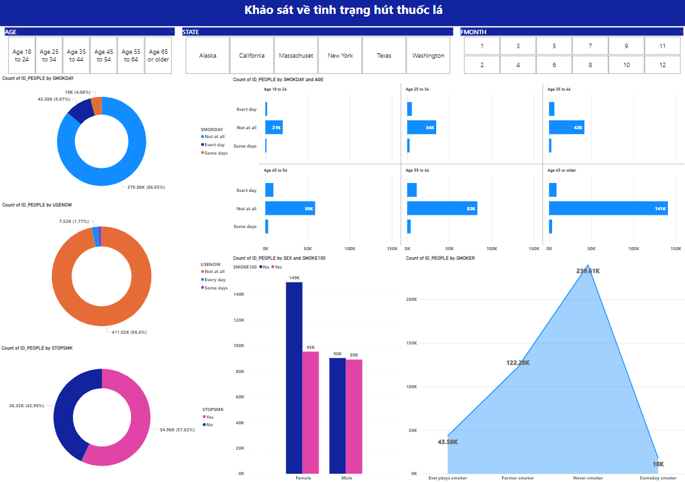
\includegraphics[scale = 0.8]{trang/dashboard3.png}
              \caption{Khảo sát về tình trạng hút thuốc lá}
            \end{figure}
    \end{center}
    Từ Dashboard này ta có được thông tin phân tích như sau
    \begin{itemize}[label= $-$]
        \item Số lượng người hút thuốc mỗi ngày chiếm 9,87\% còn lại là số lượng người chưa hút thuốc hoặc hút ít.
        
        \item Thói quen hút thuốc theo nhóm tuổi: số lượng người hút thuốc mỗi ngày ở nhóm từ 45 đến 54 tuổi và từ 55 đến 64 tuổi là đông hơn so với các nhóm còn lại.
        
        \item Số lượng người cố gắng bỏ thuốc chiếm 57,02\% so với những người chưa có ý định đó.
        
        \item Ở nữ thì việc hút ít hơn 100 điếu có số lượng nhiều hơn hắn so với việc hút nhiều hơn 100 điếu. Còn ở nam thì việc hút ít hơn hay nhiều hơn 100 điếu là ngang nhau và ngang với số người nữ hút nhiều hơn 100 điếu.
        
        \item Cuối cùng là số lượng người hút thuốc theo tấn suất thì ở đây ngoài việc không sử dụng là chủ yếu thì tiếp đến là người đã từng sử dụng chiếm khoảng $\frac{1}{3}$ tổng người tham gia, sau đó mới đến người hút hàng ngày và hút ít.
    \end{itemize}
    Qua đó, ta thấy trong những người tham gia thực hiện khảo sát này thì số người sử dụng thuốc lá là không nhiều.
\end{enumerate}

\subsubsection{Bài học tổng kết}
Sau khi cùng nhau tìm hiểu và hoàn thành bài tập nhóm này, nhóm chúng em đã rút ra được một số bài học như sau
\begin{enumerate}
    \item Cần tìm hiểu kĩ về chuyên môn, nghiệp vụ và các quá trình liên quan trước khi phân tích thiết kế và xây dựng Datawarehouse

    \item Kích thước dữ liệu lớn cần phải import và ETL sao cho hợp lý
    
    \item Dữ liệu trong thực tế không bao giờ hoàn hảo, luôn có các trường cần xử lý
    
    \item Data model phải có quan hệ giữa các bảng, thông tin như khoá chính, kiểu dữ liệu,...
    
    \item Dashboard phải bám sát nghiệp vụ, đảm bảo tính đa dạng, trực quan, có các thành phần như: footer, header, slicer,...
    
    \item Dashboard phải mang tính phân tích, so sánh, không quá tập trung vào thống kê, miêu tả.
\end{enumerate}



%\newpage
%\section{Tiền xử lý dữ liệu}
Dữ liệu gốc chứa gần 1,5 triệu bản ghi các dữ liệu đều đã được mã hóa dưới dạng số. Tha thực hiện ETL dữ liệu bằng Excel  gồm các thao tác như thay thế giá trị , đổi kiểu dữ liệu , tách cột , xử lý các cột ngày tháng 
Đầu tiên đưa dữ liệu vào Power query .Nhận thấy có 3 file dữ liệu của năm 2013 , 2014, 2015 đều có các cột tương ứng giống nhau . Để giúp cho việc thống kê và báo cáo được dễ dàng hơn  ta thực hiện nối các bảng lại với nhau bằng cách sử dụng \textbf{Append Quieries } .
\\\textbf{Xử lý dữ liệu mã hóa }
Các dữ liệu trong bảng 2013, 2014,2015 đều đã được mã hóa dưới dạng số. Do đó cần phải giải mã chúng để đưa về các giá trị cụ thể chi tiết hơn. Có rất nhiều cách để giải mã như tách cột, thêm cột, thêm cột có
điều kiện, thay thế giá trị, .... Cụ thể:
\begin{itemize}
    \item Giải mã dữ liệu cột IDAY , IMOUNTH , IYEAR \\\hfill
    Nhận thấy dữ liệu trong các cột IDAY, IMOUTH ,IYEAR đều được bao bọc bởi cặp dấu \textbf{''} do đó cần phải tách dữ liệu ra bằng cách xử dụng \textbf{Split Column } với dấu phân cách là \textbf{'}. Ta thu được kết quả như hình dưới :
    
            \begin{figure}[!h]
                \begin{center}
                \includegraphics[scale = 0.8]{HONG/2.png}
              \caption{Khảo sát về khả năng tiếp cận y tế}
         
\end{center}
   \end{figure}
   Sau khi đã tách dữ liệu của 3 cột ta thực hiện xóa các cột IMONTH.1,IMONTH.3 , IYEAR.1 ,IYEAR.3 ,IDAY.1 ,IDAY.3 bởi vì các cột này đều không có giá trị sử dụng . Thực hiện gộp các cột IDAY.2 , IMONTH.2 ,IYEAR.2    với nhau bằng cách sử dụng\textit{ merge columns} với seperator là / , sau đó chuyển dữ liệu về dạng ngày tháng ta thu được kết quả như hình dưới đây :
    \begin{figure}[!h]
                \begin{center}
                \includegraphics[scale = 0.8]{HONG/3.png}
              \caption{Khảo sát về khả năng tiếp cận y tế}
         
\end{center}
   \end{figure}
   \item Giải mã hóa các cột giá trị khác 
   Thực hiện thay thế các giá trị số thành các giá trị cụ thể ví dụ như ở cột \textbf{SEX} chỉ có 2 giá trị số là 1 và 2 , nhìn vào giá trị ta không thể biết được nó có nghĩa là gì do đó ta cần giải mã nó với 1 tương ứng là\textit{ male} , với 2 tương ứng là\textit{ female }.
   Thực hiện giải mã bằng cách thay thế giá trị (sử dụng replace values ) hoặc megre quieres bảng gốc với bảng dữ liệu giải mã tương ứng . Tuy nhiên khi dữ liệu bị mã hóa có nhiều việc thay thế giá trị sẽ rất là tốn thời gian do đó ta thực hiện merge quieres thu được kết quả như hình dưới
     \begin{figure}[!h]
                \begin{center}
                \includegraphics[scale = 0.8]{HONG/5.png}
                \end{center}
    \end{figure}
\end{itemize}
\textbf{Xóa các giá trị null trong bảng }
Thực hiện xóa các giá trị null ở mỗi bảng .Các giá trị này sẽ làm cho việc báo cáo thống kê phức  tạp do đó ta cần thực thao tác xóa . Dưới đây là kết quả của quá trình xóa các giá trị null trong cột \textbf{LASTSMK2} :
 
            \begin{figure}[!h]
                \begin{center}
                \includegraphics[scale = 0.8]{HONG/1.png}
              \caption{Khảo sát về khả năng tiếp cận y tế}
         
\end{center}
   \end{figure}
\begin{itemize}
\item Tách các sheet theo từng chủ đề :

\begin{itemize}
    \item PeopleInfor: Thông tin cá nhân của người tham gia khảo sát.
    \item PeopleHealth: Tình trạng sức khỏe của người tham gia khảo sát.
\item SmokeStatus: Tình trạng hút thuốc của người tham gia khảo sát.
\item Date: Ngày khảo sát.
\end{itemize} 
\item Xử lí dữ liệu mã hóa: Sử dụng các công cụ như tách cột, thêm cột, thêm cột có
điều kiện, thay thế giá trị, ... để thay các giá trị mã hóa thành các thông tin có ý
nghĩa.
\item Các dữ liệu bị mã hóa có nhiều hơn 5 giá trị được thống kê thành các bảng thông
tin.
\end{itemize}
Lưu dữ liệu vào cơ sở dữ liệu:

\begin{itemize}
    \item Dữ liệu sau khi được xử lí đơn giản được lưu vào CSDL HealthCare, vùng dữ liệu
được lưu này gọi là Stagging, là vùng đệm chứa dữ liệu trước khi đưa vào kho dữ liệu.
\item Xây dựng kho dữ liệu bằng cách tạo các bảng trong cơ sở dữ liệu theo mô hình OLAP
đã được thiết kế.

\end{itemize}
Đổ dữ liệu từ cơ sở dữ liệu vào kho dữ liệu:
\begin{itemize}
    \item Các dữ liệu cố định, không thay đổi theo thời gian sẽ được chuyển trực tiếp từ
Stagging vào Kho dữ liệu thông qua câu lệnh “Insert”
\item Đối với các dữ liệu được cập nhật định kì theo thời gian (tức là cứ sau một khoảng
thời gian sẽ có dữ liệu) mới được thêm vào thì việc cứ mỗi lần phải viết lại câu lệnh
“Insert” là rất mất thời gian. Thay vào đó, ta sẽ đưa câu lệnh “Insert” tạo thành một
thủ tục để mỗi lần cập nhật dữ liệu ta chỉ cần gọi thủ thục một cách nhanh chóng.
\begin{itemize}
    \item Thủ tục đổ dữ liệu vào các bảng Dim
\end{itemize} 
\end{itemize}

\newpage
\input{contents/Chapter cuối}
\end{document} 
